\documentclass[a4paper,11pt]{article}

% ─── Page Setup ────────────────────────────────────────────────────
\usepackage[margin=1.2cm, top=0.8cm, bottom=1cm]{geometry}
\usepackage{graphicx}
\usepackage{xcolor}
\usepackage{tikz}
\usetikzlibrary{shapes.geometric, arrows.meta, positioning, calc, fit, backgrounds}
\usepackage{tcolorbox}
\tcbuselibrary{skins, breakable, raster, shadows}
\usepackage{amsmath,amssymb}
\usepackage{booktabs}
\usepackage{multicol}
\usepackage{enumitem}
\usepackage{fontenc}
\usepackage{tgheros}
\renewcommand{\familydefault}{\sfdefault}
\usepackage{array}
\usepackage{colortbl}
\usepackage{tabularx}
\usepackage{setspace}
\usepackage{hyperref}
\hypersetup{colorlinks=false}

\pagestyle{empty}
\setlength{\parindent}{0pt}
\setlength{\parskip}{4pt}

% ─── Color Palette (Modern UI) ─────────────────────────────────────
\definecolor{primary}{HTML}{0F172A}      % Slate 900
\definecolor{secondary}{HTML}{475569}    % Slate 600
\definecolor{accent}{HTML}{F59E0B}       % Amber 500
\definecolor{accentlight}{HTML}{FEF3C7}  % Amber 100
\definecolor{success}{HTML}{10B981}      % Emerald 500
\definecolor{successlight}{HTML}{D1FAE5} % Emerald 100
\definecolor{danger}{HTML}{E11D48}       % Rose 600
\definecolor{dangerlight}{HTML}{FFE4E6}  % Rose 100
\definecolor{info}{HTML}{0EA5E9}         % Sky 500
\definecolor{infolight}{HTML}{E0F2FE}    % Sky 100
\definecolor{purple}{HTML}{8B5CF6}       % Violet 500
\definecolor{purplelight}{HTML}{EDE9FE}  % Violet 100
\definecolor{headerbg}{HTML}{0F172A}     % Header background
\definecolor{headertext}{HTML}{F8FAFC}   % Slate 50
\definecolor{cardbg}{HTML}{FFFFFF}       % Card background
\definecolor{pagebg}{HTML}{F8FAFC}       % Slate 50 page bg
\definecolor{gridbg}{HTML}{BBAA99}       % 2048 grid bg
\definecolor{tile2}{HTML}{EEE4DA}
\definecolor{tile4}{HTML}{EDE0C8}
\definecolor{tile8}{HTML}{F2B179}
\definecolor{tile16}{HTML}{F59563}
\definecolor{tile32}{HTML}{F67C5F}
\definecolor{tile64}{HTML}{F65E3B}
\definecolor{tile128}{HTML}{EDCF72}
\definecolor{tile256}{HTML}{EDCC61}
\definecolor{tile512}{HTML}{EDC850}
\definecolor{tile1024}{HTML}{EDC53F}
\definecolor{tile2048}{HTML}{EDC22E}

% ─── Box Styles ────────────────────────────────────────────────────
\newtcolorbox{headerbox}{
    enhanced, colback=headerbg, colframe=headerbg,
    coltext=headertext, fontupper=\bfseries\large,
    boxrule=0pt, arc=8pt, left=10pt, right=10pt,
    top=8pt, bottom=8pt,
    drop fuzzy shadow=black!30
}

\newtcolorbox{sectionbox}[2][]{
    enhanced, colback=cardbg, colframe=#2,
    title style={left color=#2, right color=#2!75!cardbg},
    coltitle=white, fonttitle=\bfseries\large,
    title=#1, boxrule=1.5pt, arc=6pt,
    left=8pt, right=8pt, top=6pt, bottom=6pt,
    drop fuzzy shadow=black!10,
    toptitle=5pt, bottomtitle=5pt,
}

\newtcolorbox{highlightbox}[1][accent]{
    enhanced, colback=#1!8, colframe=#1,
    boxrule=2pt, arc=4pt, left=8pt, right=8pt,
    top=4pt, bottom=4pt,
}

\newtcolorbox{calloutbox}[1][info]{
    enhanced, colback=#1!6, colframe=#1!60,
    boxrule=0pt, arc=4pt, left=8pt, right=8pt,
    top=4pt, bottom=4pt, borderline west={4pt}{0pt}{#1},
}

\newtcolorbox{keybox}{
    enhanced, colback=accent!10, colframe=accent,
    boxrule=2pt, arc=8pt, left=10pt, right=10pt,
    top=8pt, bottom=8pt,
    fontupper=\large,
    drop fuzzy shadow=accent!20
}

% ─── Macros ────────────────────────────────────────────────────────
\newcommand{\pagetitle}[2]{%
\begin{headerbox}
\begin{center}
{\fontsize{20}{24}\selectfont #1}\\[3pt]
{\normalsize\normalfont\color{white!80} #2}
\end{center}
\end{headerbox}
\vspace{6pt}
}

\newcommand{\pageheader}{%
\begin{tikzpicture}[remember picture, overlay]
\fill[pagebg] (current page.north west) rectangle (current page.south east);
\end{tikzpicture}%
}

\newcommand{\statico}[1]{\textcolor{accent}{\textbf{#1}}}
\newcommand{\agentname}[1]{\textcolor{primary}{\textbf{#1}}}

% ═══════════════════════════════════════════════════════════════════
% PAGE 1: PROBLEM & MDP
% ═══════════════════════════════════════════════════════════════════
\begin{document}
\pageheader

% ─── Title Banner ──────────────────────────────────────────────────

\begin{tikzpicture}
\fill[primary, rounded corners=8pt] (0,0) rectangle (\textwidth, 2.8cm);
\node[anchor=center, text=white] at (0.5\textwidth, 1.9cm) {
    {\fontsize{22}{26}\selectfont\bfseries Solving 2048: Classical RL vs.\ LLM-Guided RLVR}
};
\node[anchor=center, text=white!85] at (0.5\textwidth, 1.05cm) {
    {\large CS 5180 --- Reinforcement Learning \quad|\quad Northeastern University}
};
\node[anchor=center, text=accent] at (0.5\textwidth, 0.4cm) {
    {\normalsize\bfseries Shriman Raghav \quad\&\quad Gautham Ramkumar \quad|\quad MS Robotics}
};
\end{tikzpicture}
\vspace{6pt}

\begin{multicols}{2}

% ─── Game Visual ───────────────────────────────────────────────────
\begin{sectionbox}[{\raisebox{-1pt}{\tikz\fill[accent] (0,0) rectangle (0.35,0.35);}\; The 2048 Puzzle}]{accent}

\begin{center}
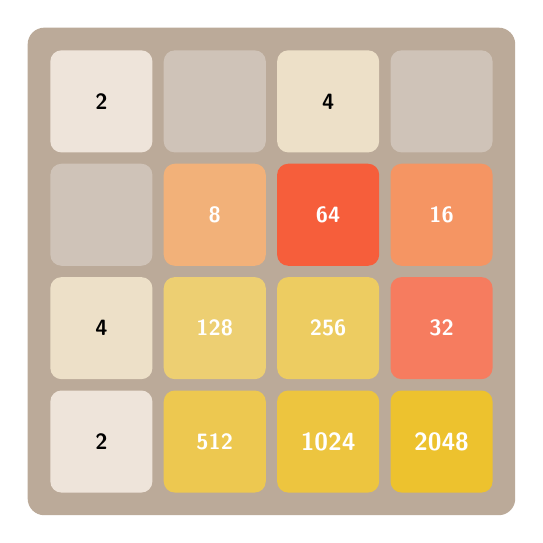
\begin{tikzpicture}[scale=0.72]
% Grid background
\fill[gridbg, rounded corners=6pt] (-0.3,-0.3) rectangle (8.3,8.3);
% Row 3 (top)
\fill[tile2, rounded corners=4pt] (0.1,6.1) rectangle (1.9,7.9); \node[font=\bfseries\footnotesize] at (1,7) {2};
\fill[gridbg!70, rounded corners=4pt] (2.1,6.1) rectangle (3.9,7.9);
\fill[tile4, rounded corners=4pt] (4.1,6.1) rectangle (5.9,7.9); \node[font=\bfseries\footnotesize] at (5,7) {4};
\fill[gridbg!70, rounded corners=4pt] (6.1,6.1) rectangle (7.9,7.9);
% Row 2
\fill[gridbg!70, rounded corners=4pt] (0.1,4.1) rectangle (1.9,5.9);
\fill[tile8, rounded corners=4pt] (2.1,4.1) rectangle (3.9,5.9); \node[font=\bfseries\footnotesize, text=white] at (3,5) {8};
\fill[tile64, rounded corners=4pt] (4.1,4.1) rectangle (5.9,5.9); \node[font=\bfseries\footnotesize, text=white] at (5,5) {64};
\fill[tile16, rounded corners=4pt] (6.1,4.1) rectangle (7.9,5.9); \node[font=\bfseries\footnotesize, text=white] at (7,5) {16};
% Row 1
\fill[tile4, rounded corners=4pt] (0.1,2.1) rectangle (1.9,3.9); \node[font=\bfseries\footnotesize] at (1,3) {4};
\fill[tile128, rounded corners=4pt] (2.1,2.1) rectangle (3.9,3.9); \node[font=\bfseries\footnotesize, text=white] at (3,3) {128};
\fill[tile256, rounded corners=4pt] (4.1,2.1) rectangle (5.9,3.9); \node[font=\bfseries\footnotesize, text=white] at (5,3) {256};
\fill[tile32, rounded corners=4pt] (6.1,2.1) rectangle (7.9,3.9); \node[font=\bfseries\footnotesize, text=white] at (7,3) {32};
% Row 0 (bottom)
\fill[tile2, rounded corners=4pt] (0.1,0.1) rectangle (1.9,1.9); \node[font=\bfseries\footnotesize] at (1,1) {2};
\fill[tile512, rounded corners=4pt] (2.1,0.1) rectangle (3.9,1.9); \node[font=\bfseries\footnotesize, text=white] at (3,1) {512};
\fill[tile1024, rounded corners=4pt] (4.1,0.1) rectangle (5.9,1.9); \node[font=\bfseries\small, text=white] at (5,1) {1024};
\fill[tile2048, rounded corners=4pt] (6.1,0.1) rectangle (7.9,1.9); \node[font=\bfseries\small, text=white] at (7,1) {2048};
\end{tikzpicture}
\end{center}

\vspace{2pt}
{\small Slide tiles in 4 directions. Equal tiles merge, doubling their value. Reach \textbf{2048} to win! Random new tiles (2 or 4) spawn after each valid move.}
\end{sectionbox}

% ─── Why It's Hard ─────────────────────────────────────────────────
\begin{sectionbox}[{\raisebox{-1pt}{\tikz\fill[danger] (0,0) rectangle (0.35,0.35);}\; Why 2048 Is Hard for RL}]{danger}
\begin{itemize}[nosep, leftmargin=12pt, itemsep=3pt]
    \item[\textcolor{danger}{\textbullet}] \textbf{Sparse rewards} --- hundreds of low-value merges before one big payoff
    \item[\textcolor{danger}{\textbullet}] \textbf{Stochastic dynamics} --- random tile spawns prevent deterministic planning
    \item[\textcolor{danger}{\textbullet}] \textbf{Huge state space} --- $\sim\!17^{16} \approx 2.8 \times 10^{19}$ configurations
    \item[\textcolor{danger}{\textbullet}] \textbf{Long horizons} --- episodes last 100--1000+ steps
\end{itemize}
\end{sectionbox}

\columnbreak

% ─── MDP Diagram ───────────────────────────────────────────────────
\begin{sectionbox}[{\raisebox{-1pt}{\tikz\fill[info] (0,0) rectangle (0.35,0.35);}\; Formal MDP}]{info}

\begin{center}
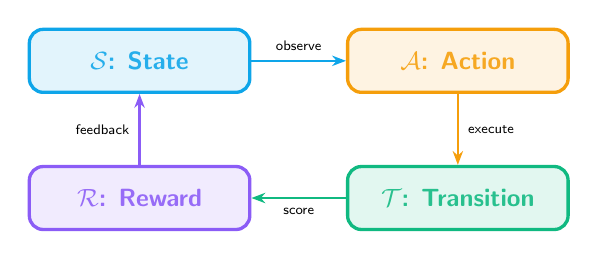
\begin{tikzpicture}[
    node distance=0.9cm and 1.2cm,
    block/.style={rectangle, rounded corners=5pt, draw=#1, fill=#1!12,
                  minimum width=2.8cm, minimum height=0.8cm, font=\small\bfseries,
                  text=#1!90, line width=1.2pt},
    arr/.style={-{Stealth[length=5pt]}, thick, #1},
    label/.style={font=\tiny, text=#1, align=center}
]
% Nodes
\node[block=info] (S) {$\mathcal{S}$: State};
\node[block=accent, right=of S] (A) {$\mathcal{A}$: Action};
\node[block=success, below=of A] (T) {$\mathcal{T}$: Transition};
\node[block=purple, below=of S] (R) {$\mathcal{R}$: Reward};

% Arrows
\draw[arr=info] (S) -- (A) node[midway, above, label=black] {observe};
\draw[arr=accent] (A) -- (T) node[midway, right, label=black] {execute};
\draw[arr=success] (T) -- (R) node[midway, below, label=black] {score};
\draw[arr=purple] (R) -- (S) node[midway, left, label=black] {feedback};
\end{tikzpicture}
\end{center}

\vspace{2pt}
\renewcommand{\arraystretch}{1.25}
{\small
\begin{tabularx}{\linewidth}{@{}>{\bfseries\color{info}}l X@{}}
$\mathcal{S}$ & $4{\times}4$ board $\to$ 16-channel binary tensor $\mathbf{x} \in \{0,1\}^{16 \times 4 \times 4}$ \\
$\mathcal{A}$ & \{UP, RIGHT, DOWN, LEFT\} --- 4 discrete actions \\
$\mathcal{T}$ & Slide-merge (deterministic) $\oplus$ random tile spawn (stochastic: 2 w/ $p{=}0.9$, 4 w/ $p{=}0.1$) \\
$\mathcal{R}$ & Merge score delta + milestone bonuses (+50@256, +100@512, +200@1024) \\
$\gamma$ & 0.99 \\
\end{tabularx}
}
\end{sectionbox}

% ─── Observation Encoding ──────────────────────────────────────────
\begin{sectionbox}[{\raisebox{-1pt}{\tikz\fill[success] (0,0) rectangle (0.35,0.35);}\; Observation Encoding}]{success}

\begin{center}
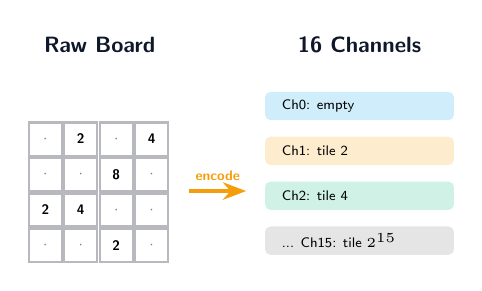
\begin{tikzpicture}[scale=0.6]
% Board
\node[font=\footnotesize\bfseries, text=primary] at (1.5, 4.6) {Raw Board};
% Manual 4x4 grid
\draw[primary!30, thick] (0,2.25) rectangle (0.7,2.95); \node[font=\tiny, text=gray] at (0.35,2.6) {$\cdot$};
\draw[primary!30, thick] (0.75,2.25) rectangle (1.45,2.95); \node[font=\tiny\bfseries] at (1.1,2.6) {2};
\draw[primary!30, thick] (1.5,2.25) rectangle (2.2,2.95); \node[font=\tiny, text=gray] at (1.85,2.6) {$\cdot$};
\draw[primary!30, thick] (2.25,2.25) rectangle (2.95,2.95); \node[font=\tiny\bfseries] at (2.6,2.6) {4};
\draw[primary!30, thick] (0,1.5) rectangle (0.7,2.2); \node[font=\tiny, text=gray] at (0.35,1.85) {$\cdot$};
\draw[primary!30, thick] (0.75,1.5) rectangle (1.45,2.2); \node[font=\tiny, text=gray] at (1.1,1.85) {$\cdot$};
\draw[primary!30, thick] (1.5,1.5) rectangle (2.2,2.2); \node[font=\tiny\bfseries] at (1.85,1.85) {8};
\draw[primary!30, thick] (2.25,1.5) rectangle (2.95,2.2); \node[font=\tiny, text=gray] at (2.6,1.85) {$\cdot$};
\draw[primary!30, thick] (0,0.75) rectangle (0.7,1.45); \node[font=\tiny\bfseries] at (0.35,1.1) {2};
\draw[primary!30, thick] (0.75,0.75) rectangle (1.45,1.45); \node[font=\tiny\bfseries] at (1.1,1.1) {4};
\draw[primary!30, thick] (1.5,0.75) rectangle (2.2,1.45); \node[font=\tiny, text=gray] at (1.85,1.1) {$\cdot$};
\draw[primary!30, thick] (2.25,0.75) rectangle (2.95,1.45); \node[font=\tiny, text=gray] at (2.6,1.1) {$\cdot$};
\draw[primary!30, thick] (0,0) rectangle (0.7,0.7); \node[font=\tiny, text=gray] at (0.35,0.35) {$\cdot$};
\draw[primary!30, thick] (0.75,0) rectangle (1.45,0.7); \node[font=\tiny, text=gray] at (1.1,0.35) {$\cdot$};
\draw[primary!30, thick] (1.5,0) rectangle (2.2,0.7); \node[font=\tiny\bfseries] at (1.85,0.35) {2};
\draw[primary!30, thick] (2.25,0) rectangle (2.95,0.7); \node[font=\tiny, text=gray] at (2.6,0.35) {$\cdot$};

% Arrow
\draw[-{Stealth}, very thick, accent] (3.4, 1.5) -- (4.6, 1.5)
    node[midway, above, font=\tiny\bfseries] {encode};

% Channels - manual
\node[font=\footnotesize\bfseries, text=primary] at (7.0, 4.6) {16 Channels};
\fill[info!20, rounded corners=2pt] (5.0, 3.0) rectangle (9.0, 3.6);
\node[font=\tiny, anchor=west] at (5.15, 3.3) {Ch0: empty};
\fill[accent!20, rounded corners=2pt] (5.0, 2.05) rectangle (9.0, 2.65);
\node[font=\tiny, anchor=west] at (5.15, 2.35) {Ch1: tile 2};
\fill[success!20, rounded corners=2pt] (5.0, 1.1) rectangle (9.0, 1.7);
\node[font=\tiny, anchor=west] at (5.15, 1.4) {Ch2: tile 4};
\fill[gray!20, rounded corners=2pt] (5.0, 0.15) rectangle (9.0, 0.75);
\node[font=\tiny, anchor=west] at (5.15, 0.45) {... Ch15: tile $2^{15}$};
\end{tikzpicture}
\end{center}

\vspace{-2pt}
{\small $x_{k,i,j}=\mathbb{1}[B_{i,j}=2^k]$ --- one-hot power-of-2 avoids magnitude bias in CNN filters.}
\end{sectionbox}

\end{multicols}

% ─── Bottom Banner ─────────────────────────────────────────────────
\begin{keybox}
\begin{center}
{\large\bfseries 9 Agents} benchmarked end-to-end \quad\textbullet\quad
{\large\bfseries 5M training steps} per agent \quad\textbullet\quad
{\large\bfseries DQN reaches tile 2048}
\end{center}
\end{keybox}

% ═══════════════════════════════════════════════════════════════════
% PAGE 2: ALGORITHMS
% ═══════════════════════════════════════════════════════════════════
\newpage
\pageheader

\pagetitle{Algorithms \& Architecture}{Shared CNN backbone isolates the learning algorithm --- not the architecture}

\begin{multicols}{2}

% ─── CNN Architecture ──────────────────────────────────────────────
\begin{sectionbox}[{\raisebox{-1pt}{\tikz\fill[primary] (0,0) rectangle (0.35,0.35);}\; Shared CNN Backbone (330K params)}]{primary}

\begin{center}
\resizebox{\linewidth}{!}{
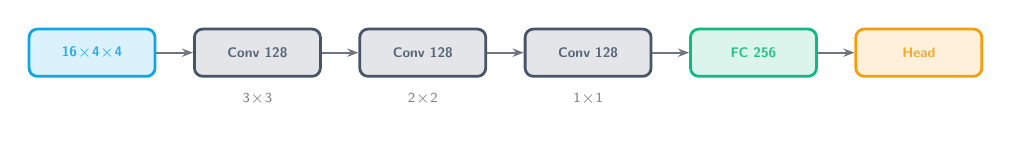
\begin{tikzpicture}[
    layer/.style={rectangle, rounded corners=3pt, draw=#1, fill=#1!15,
                  minimum width=1.6cm, minimum height=0.6cm, font=\tiny\bfseries,
                  text=#1!90, line width=1pt},
    arr/.style={-{Stealth[length=4pt]}, thick, primary!60}
]
\node[layer=info] (input) at (0,0) {16$\times$4$\times$4};
\node[layer=secondary] (c1) at (2.1,0) {Conv 128};
\node[layer=secondary] (c2) at (4.2,0) {Conv 128};
\node[layer=secondary] (c3) at (6.3,0) {Conv 128};
\node[layer=success] (fc) at (8.4,0) {FC 256};
\node[layer=accent] (out) at (10.5,0) {Head};

\draw[arr] (input) -- (c1);
\draw[arr] (c1) -- (c2);
\draw[arr] (c2) -- (c3);
\draw[arr] (c3) -- (fc);
\draw[arr] (fc) -- (out);

\node[font=\tiny, text=gray, below=2pt of c1] {3$\times$3};
\node[font=\tiny, text=gray, below=2pt of c2] {2$\times$2};
\node[font=\tiny, text=gray, below=2pt of c3] {1$\times$1};
\end{tikzpicture}
}
\end{center}

{\small Three 2$\times$2 convolutions (128 filters each) + ReLU $\to$ 256-dim features. Each algorithm adds its own task head. All deep agents share this \textbf{identical} backbone.}
\end{sectionbox}

% ─── DQN ───────────────────────────────────────────────────────────
\begin{sectionbox}[{\raisebox{-1pt}{\tikz\fill[tile2048] (0,0) rectangle (0.35,0.35);}\; \statico{DQN} $|$ Best Performer $\bigstar$}]{accent}

\begin{center}
\resizebox{\linewidth}{!}{
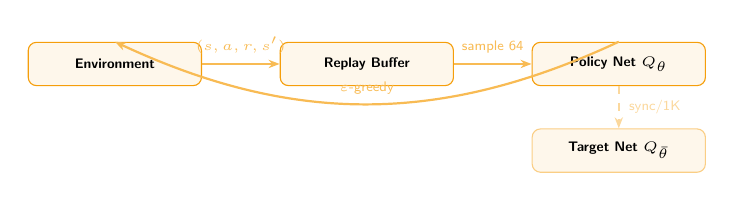
\begin{tikzpicture}[
    box/.style={rectangle, rounded corners=3pt, draw=accent, fill=accent!8,
                minimum width=2.2cm, minimum height=0.55cm, font=\tiny\bfseries},
    arr/.style={-{Stealth[length=4pt]}, thick, accent!70}
]
\node[box] (env) at (0,0) {Environment};
\node[box] (buf) at (3.2,0) {Replay Buffer};
\node[box] (pol) at (6.4,0) {Policy Net $Q_\theta$};
\node[box, draw=accent!50] (tgt) at (6.4,-1.1) {Target Net $Q_{\bar\theta}$};

\draw[arr] (env) -- (buf) node[midway, above, font=\tiny] {$(s,a,r,s')$};
\draw[arr] (buf) -- (pol) node[midway, above, font=\tiny] {sample 64};
\draw[arr, dashed, accent!40] (pol) -- (tgt) node[midway, right, font=\tiny] {sync/1K};
\draw[arr, bend left=25] (pol.north) to node[above, font=\tiny] {$\varepsilon$-greedy} (env.north);
\end{tikzpicture}
}
\end{center}

{\small
$\mathcal{L}=\text{SmoothL1}\!\left(Q_\theta(s,a),\; r+\gamma\max_{a'}Q_{\bar\theta}(s',a')\right)$

\textbf{Key:} Buffer 100K, $\varepsilon$: $1.0 \to 0.01$ over 100K steps, lr $10^{-4}$, grad clip 1.0
}
\end{sectionbox}

% ─── PPO ───────────────────────────────────────────────────────────
\begin{sectionbox}[{\raisebox{-1pt}{\tikz\fill[info] (0,0) rectangle (0.35,0.35);}\; \agentname{PPO} $|$ MaskablePPO}]{info}
{\small
Clipped surrogate with invalid-action masking:

$\mathcal{L}=\min\!\left(r_t\hat{A}_t,\;\text{clip}(r_t,1{\pm}0.2)\hat{A}_t\right)$

GAE $\lambda{=}0.95$, 2048 steps/rollout, 10 epochs/batch, 8 parallel envs. Logits $\to -\infty$ for invalid actions.
}
\end{sectionbox}

% ─── A2C ───────────────────────────────────────────────────────────
\begin{sectionbox}[{\raisebox{-1pt}{\tikz\fill[success] (0,0) rectangle (0.35,0.35);}\; \agentname{A2C} $|$ MaskableA2C}]{success}
{\small
$\mathcal{L}=-\mathbb{E}[\log\pi\hat{A}]+0.5\|R\!-\!V\|^2-0.01\,\mathcal{H}[\pi]$

5-step bootstrap, entropy reg.\ for exploration, 8 parallel envs.
}
\end{sectionbox}

\columnbreak

% ─── QR-DQN ────────────────────────────────────────────────────────
\begin{sectionbox}[{\raisebox{-1pt}{\tikz\fill[purple] (0,0) rectangle (0.35,0.35);}\; \agentname{QR-DQN} $|$ Distributional RL}]{purple}
{\small
Learns 50 quantiles of the return distribution:

$\mathcal{L}_{\text{QR}}=\frac{1}{50}\sum_i\mathbb{E}_j[\rho_{\tau_i}^\kappa(\delta_{ij})]$

Net outputs $4\!\times\!50{=}200$ values. Action by mean Q.
}
\end{sectionbox}

% ─── SAC ───────────────────────────────────────────────────────────
\begin{sectionbox}[{\raisebox{-1pt}{\tikz\fill[danger] (0,0) rectangle (0.35,0.35);}\; \agentname{SAC} $|$ Max-Entropy}]{danger}
{\small
$J(\pi)=\sum_t\mathbb{E}[r_t+\alpha\mathcal{H}[\pi(\cdot|s_t)]]$

Twin Q-nets, auto-tuned temperature $\alpha$, Polyak $\tau{=}0.005$.
}
\end{sectionbox}

% ─── LFA ───────────────────────────────────────────────────────────
\begin{sectionbox}[{\raisebox{-1pt}{\tikz\fill[success] (0,0) rectangle (0.35,0.35);}\; \agentname{LFA} $|$ Only 108 Parameters!}]{success}

\begin{calloutbox}[success]
{\bfseries\small Surprise: 108 params beats 330K--494M deep nets!}
\end{calloutbox}

\vspace{2pt}
{\small
$\hat{q}(s,a)=\mathbf{w}_a^\top\phi(s)$, \quad $\mathbf{w}\in\mathbb{R}^{4\times 27}$

\textbf{27-dim features:} log-tile values, empty ratio, merge potential, 4 monotonicity scores, corner bonus, tile distribution stats.

Semi-gradient SARSA: $\mathbf{w}_a \leftarrow \mathbf{w}_a + \alpha\delta\phi(s)$
}
\end{sectionbox}

% ─── GRPO ──────────────────────────────────────────────────────────
\begin{sectionbox}[{\raisebox{-1pt}{\tikz\fill[purple] (0,0) rectangle (0.35,0.35);}\; \agentname{GRPO} $|$ LLM + Verifiable Rewards}]{purple}

\begin{center}
\resizebox{\linewidth}{!}{
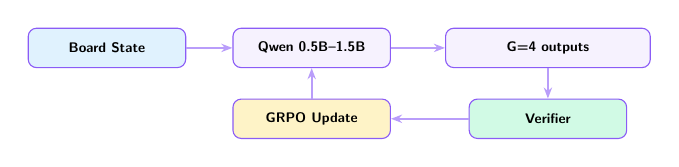
\begin{tikzpicture}[
    box/.style={rectangle, rounded corners=3pt, draw=purple, fill=purple!8,
                minimum width=2cm, minimum height=0.5cm, font=\tiny\bfseries},
    arr/.style={-{Stealth[length=4pt]}, thick, purple!60}
]
\node[box, fill=infolight] (prompt) at (0,0) {Board State};
\node[box] (llm) at (2.6,0) {Qwen 0.5B--1.5B};
\node[box, minimum width=2.6cm] (gen) at (5.6,0) {G=4 outputs};
\node[box, fill=successlight] (verify) at (5.6,-0.9) {Verifier};
\node[box, fill=accentlight] (grpo) at (2.6,-0.9) {GRPO Update};

\draw[arr] (prompt) -- (llm);
\draw[arr] (llm) -- (gen);
\draw[arr] (gen) -- (verify);
\draw[arr] (verify) -- (grpo);
\draw[arr] (grpo) -- (llm);
\end{tikzpicture}
}
\end{center}

{\small
\textbf{Models:} Qwen2.5-0.5B \& 1.5B, QLoRA 4-bit, 5.2M trainable

$\hat{A}_i=(r_i-\mu_G)/\sigma_G$ \quad {\footnotesize (group-normalized, no critic!)}

\textbf{Rewards:} Format (+0.5) $|$ Direction (+0.5) $|$ Game ($\pm$2) $|$ Quality (+0.5)

\textbf{Results:} 0.5B: tile 64 $|$ \textbf{1.5B: tile 256, score 2,348}

\begin{calloutbox}[danger]
{\footnotesize\bfseries Staged scheduling required!} All rewards at once $\to$ reward hacking.
\end{calloutbox}
}
\end{sectionbox}

\end{multicols}

% ═══════════════════════════════════════════════════════════════════
% PAGE 3: RESULTS
% ═══════════════════════════════════════════════════════════════════
\newpage
\pageheader

\pagetitle{Results}{5M training steps $\cdot$ Shaped rewards $\cdot$ NVIDIA RTX 4060 GPU}

% ─── Performance Table ─────────────────────────────────────────────
\begin{sectionbox}[{\raisebox{-1pt}{\tikz\fill[primary] (0,0) rectangle (0.35,0.35);}\; Final Performance Comparison}]{primary}

\renewcommand{\arraystretch}{1.3}
\begin{center}
{\small
\begin{tabular}{@{} >{\bfseries}l r r r r r r @{}}
\toprule
\rowcolor{primary!10}
\textbf{Agent} & \textbf{Avg Score} & \textbf{Max Score} & \textbf{Max Tile} & \textbf{512+ Rate} & \textbf{1024+ Rate} & \textbf{Parameters} \\
\midrule
\rowcolor{accentlight}
DQN $\bigstar$ & \textcolor{accent}{\textbf{7,744}} & \textcolor{accent}{\textbf{39,314}} & \textcolor{accent}{\textbf{2048}} & \textcolor{accent}{\textbf{76.0\%}} & \textcolor{accent}{\textbf{31.0\%}} & 330K \\
LFA & 2,456 & 11,436 & 1024 & 6.0\% & $<$1\% & \textcolor{success}{\textbf{108}} \\
\rowcolor{purplelight}
GRPO 1.5B & \textcolor{purple}{\textbf{2,348}} & 2,348 & \textcolor{purple}{\textbf{256}} & --- & --- & 1.8B \\
A2C & 1,944 & 9,640 & 1024 & 6.0\% & $<$1\% & 330K \\
GRPO 0.5B & 1,816 & 1,816 & 128 & --- & --- & 494M \\
SAC & 1,131 & 5,566 & 512 & $<$1\% & --- & 330K \\
QR-DQN & 995 & 5,176 & 512 & $<$1\% & --- & 430K \\
\rowcolor{dangerlight}
PPO & \textcolor{danger}{962} & 4,900 & 512 & $<$1\% & --- & 330K \\
GRPO 0.5B & 704 & 704 & 64 & --- & --- & 494M \\
\bottomrule
\multicolumn{7}{@{}l}{\footnotesize GRPO: 0.5B = Qwen2.5-0.5B (3-stage); 1.5B = Qwen2.5-1.5B (3-stage). All classical agents 5M steps.}
\end{tabular}
}
\end{center}
\end{sectionbox}

\vspace{4pt}

\begin{multicols}{2}

% ─── Scaling Table ─────────────────────────────────────────────────
\begin{sectionbox}[{\raisebox{-1pt}{\tikz\fill[info] (0,0) rectangle (0.35,0.35);}\; Scaling: 1M $\to$ 5M Steps}]{info}

\begin{center}
\resizebox{\linewidth}{!}{
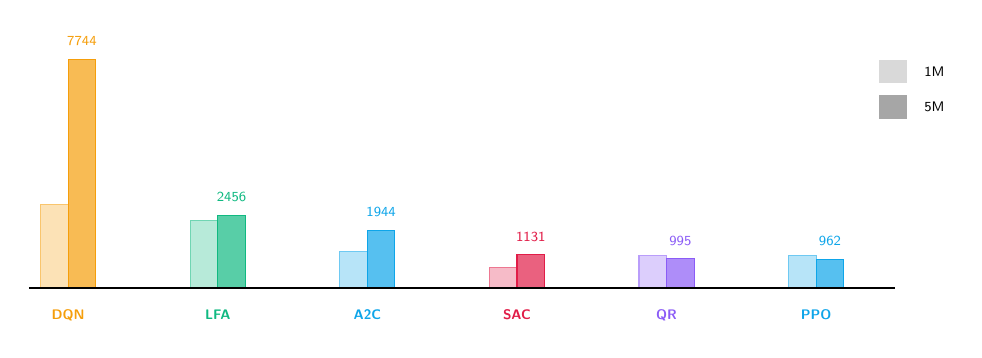
\begin{tikzpicture}
% Manual bar chart - 1M (light) and 5M (dark) side by side
\def\bw{0.35}
\def\maxval{8000}
% DQN
\fill[accent!30] (-0.35,0) rectangle (0, 1.059); \draw[accent!60] (-0.35,0) rectangle (0, 1.059);
\fill[accent!70] (0,0) rectangle (0.35, 2.904); \draw[accent] (0,0) rectangle (0.35, 2.904);
\node[font=\tiny\bfseries, anchor=north, text=accent] at (0, -0.15) {DQN};
\node[font=\tiny, anchor=south, text=accent] at (0.175, 2.95) {7744};
% LFA
\fill[success!30] (1.55,0) rectangle (1.9, 0.862); \draw[success!60] (1.55,0) rectangle (1.9, 0.862);
\fill[success!70] (1.9,0) rectangle (2.25, 0.921); \draw[success] (1.9,0) rectangle (2.25, 0.921);
\node[font=\tiny\bfseries, anchor=north, text=success] at (1.9, -0.15) {LFA};
\node[font=\tiny, anchor=south, text=success] at (2.075, 0.97) {2456};
% A2C
\fill[info!30] (3.45,0) rectangle (3.8, 0.467); \draw[info!60] (3.45,0) rectangle (3.8, 0.467);
\fill[info!70] (3.8,0) rectangle (4.15, 0.729); \draw[info] (3.8,0) rectangle (4.15, 0.729);
\node[font=\tiny\bfseries, anchor=north, text=info] at (3.8, -0.15) {A2C};
\node[font=\tiny, anchor=south, text=info] at (3.975, 0.78) {1944};
% SAC
\fill[danger!30] (5.35,0) rectangle (5.7, 0.263); \draw[danger!60] (5.35,0) rectangle (5.7, 0.263);
\fill[danger!70] (5.7,0) rectangle (6.05, 0.424); \draw[danger] (5.7,0) rectangle (6.05, 0.424);
\node[font=\tiny\bfseries, anchor=north, text=danger] at (5.7, -0.15) {SAC};
\node[font=\tiny, anchor=south, text=danger] at (5.875, 0.47) {1131};
% QR-DQN
\fill[purple!30] (7.25,0) rectangle (7.6, 0.409); \draw[purple!60] (7.25,0) rectangle (7.6, 0.409);
\fill[purple!70] (7.6,0) rectangle (7.95, 0.373); \draw[purple] (7.6,0) rectangle (7.95, 0.373);
\node[font=\tiny\bfseries, anchor=north, text=purple] at (7.6, -0.15) {QR};
\node[font=\tiny, anchor=south, text=purple] at (7.775, 0.42) {995};
% PPO
\fill[info!30] (9.15,0) rectangle (9.5, 0.412); \draw[info!60] (9.15,0) rectangle (9.5, 0.412);
\fill[info!70] (9.5,0) rectangle (9.85, 0.361); \draw[info] (9.5,0) rectangle (9.85, 0.361);
\node[font=\tiny\bfseries, anchor=north, text=info] at (9.5, -0.15) {PPO};
\node[font=\tiny, anchor=south, text=info] at (9.675, 0.41) {962};

% Legend
\fill[gray!30] (10.3, 2.6) rectangle (10.65, 2.9);
\node[font=\tiny, anchor=west] at (10.75, 2.75) {1M};
\fill[gray!70] (10.3, 2.15) rectangle (10.65, 2.45);
\node[font=\tiny, anchor=west] at (10.75, 2.3) {5M};

% Axis
\draw[thick] (-0.5, 0) -- (10.5, 0);
\end{tikzpicture}
}
\end{center}

\vspace{2pt}
\begin{calloutbox}[accent]
{\small\bfseries DQN: +174\%} scaling \quad|\quad {\small\color{danger} PPO: $-$12\%} degradation
\end{calloutbox}
\end{sectionbox}

\columnbreak

% ─── Hunt Mode ─────────────────────────────────────────────────────
\begin{sectionbox}[{\raisebox{-1pt}{\tikz\fill[success] (0,0) rectangle (0.35,0.35);}\; Hunt-2048 Mode}]{success}

\begin{center}
\resizebox{\linewidth}{!}{
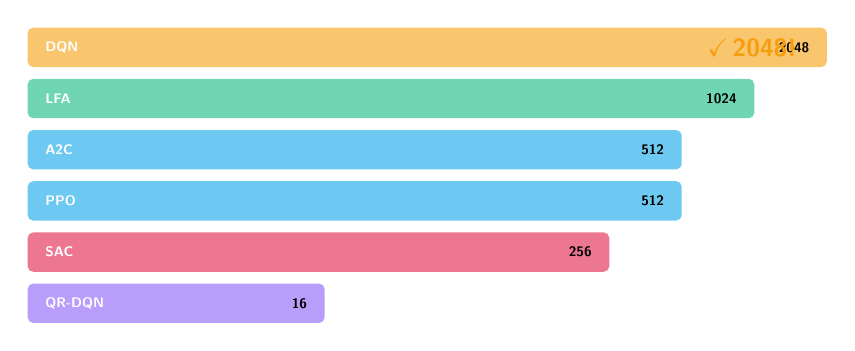
\begin{tikzpicture}
% Tile progression visualization
\foreach \i/\tile/\agent/\col in {
    0/2048/DQN/accent, 1/1024/LFA/success, 2/512/A2C/info,
    3/512/PPO/info, 4/256/SAC/danger, 5/16/QR-DQN/purple}{
    \pgfmathsetmacro{\w}{3.5 * ln(\tile+1) / ln(2049)}
    \fill[\col!60, rounded corners=2pt] (0, -\i*0.65) rectangle (\w*2.9, -\i*0.65+0.5);
    \node[font=\tiny\bfseries, anchor=west, text=white] at (0.1, -\i*0.65+0.25) {\agent};
    \node[font=\tiny\bfseries, anchor=east] at (\w*2.9-0.1, -\i*0.65+0.25) {\tile};
}
% Checkmark for DQN
\node[font=\small, text=accent] at (9.2, 0.25) {\checkmark\,\textbf{2048!}};
\end{tikzpicture}
}
\end{center}

{\small Only DQN reaches tile 2048 (score 21,572). Adding 5\% $\varepsilon$-noise breaks deterministic policy cycles.}
\end{sectionbox}
\end{multicols}

% ─── Learning Curves ───────────────────────────────────────────────
\begin{sectionbox}[{\raisebox{-1pt}{\tikz\fill[accent] (0,0) rectangle (0.35,0.35);}\; Learning Curves}]{accent}

\begin{center}
\begin{minipage}[t]{0.16\linewidth}
\centering
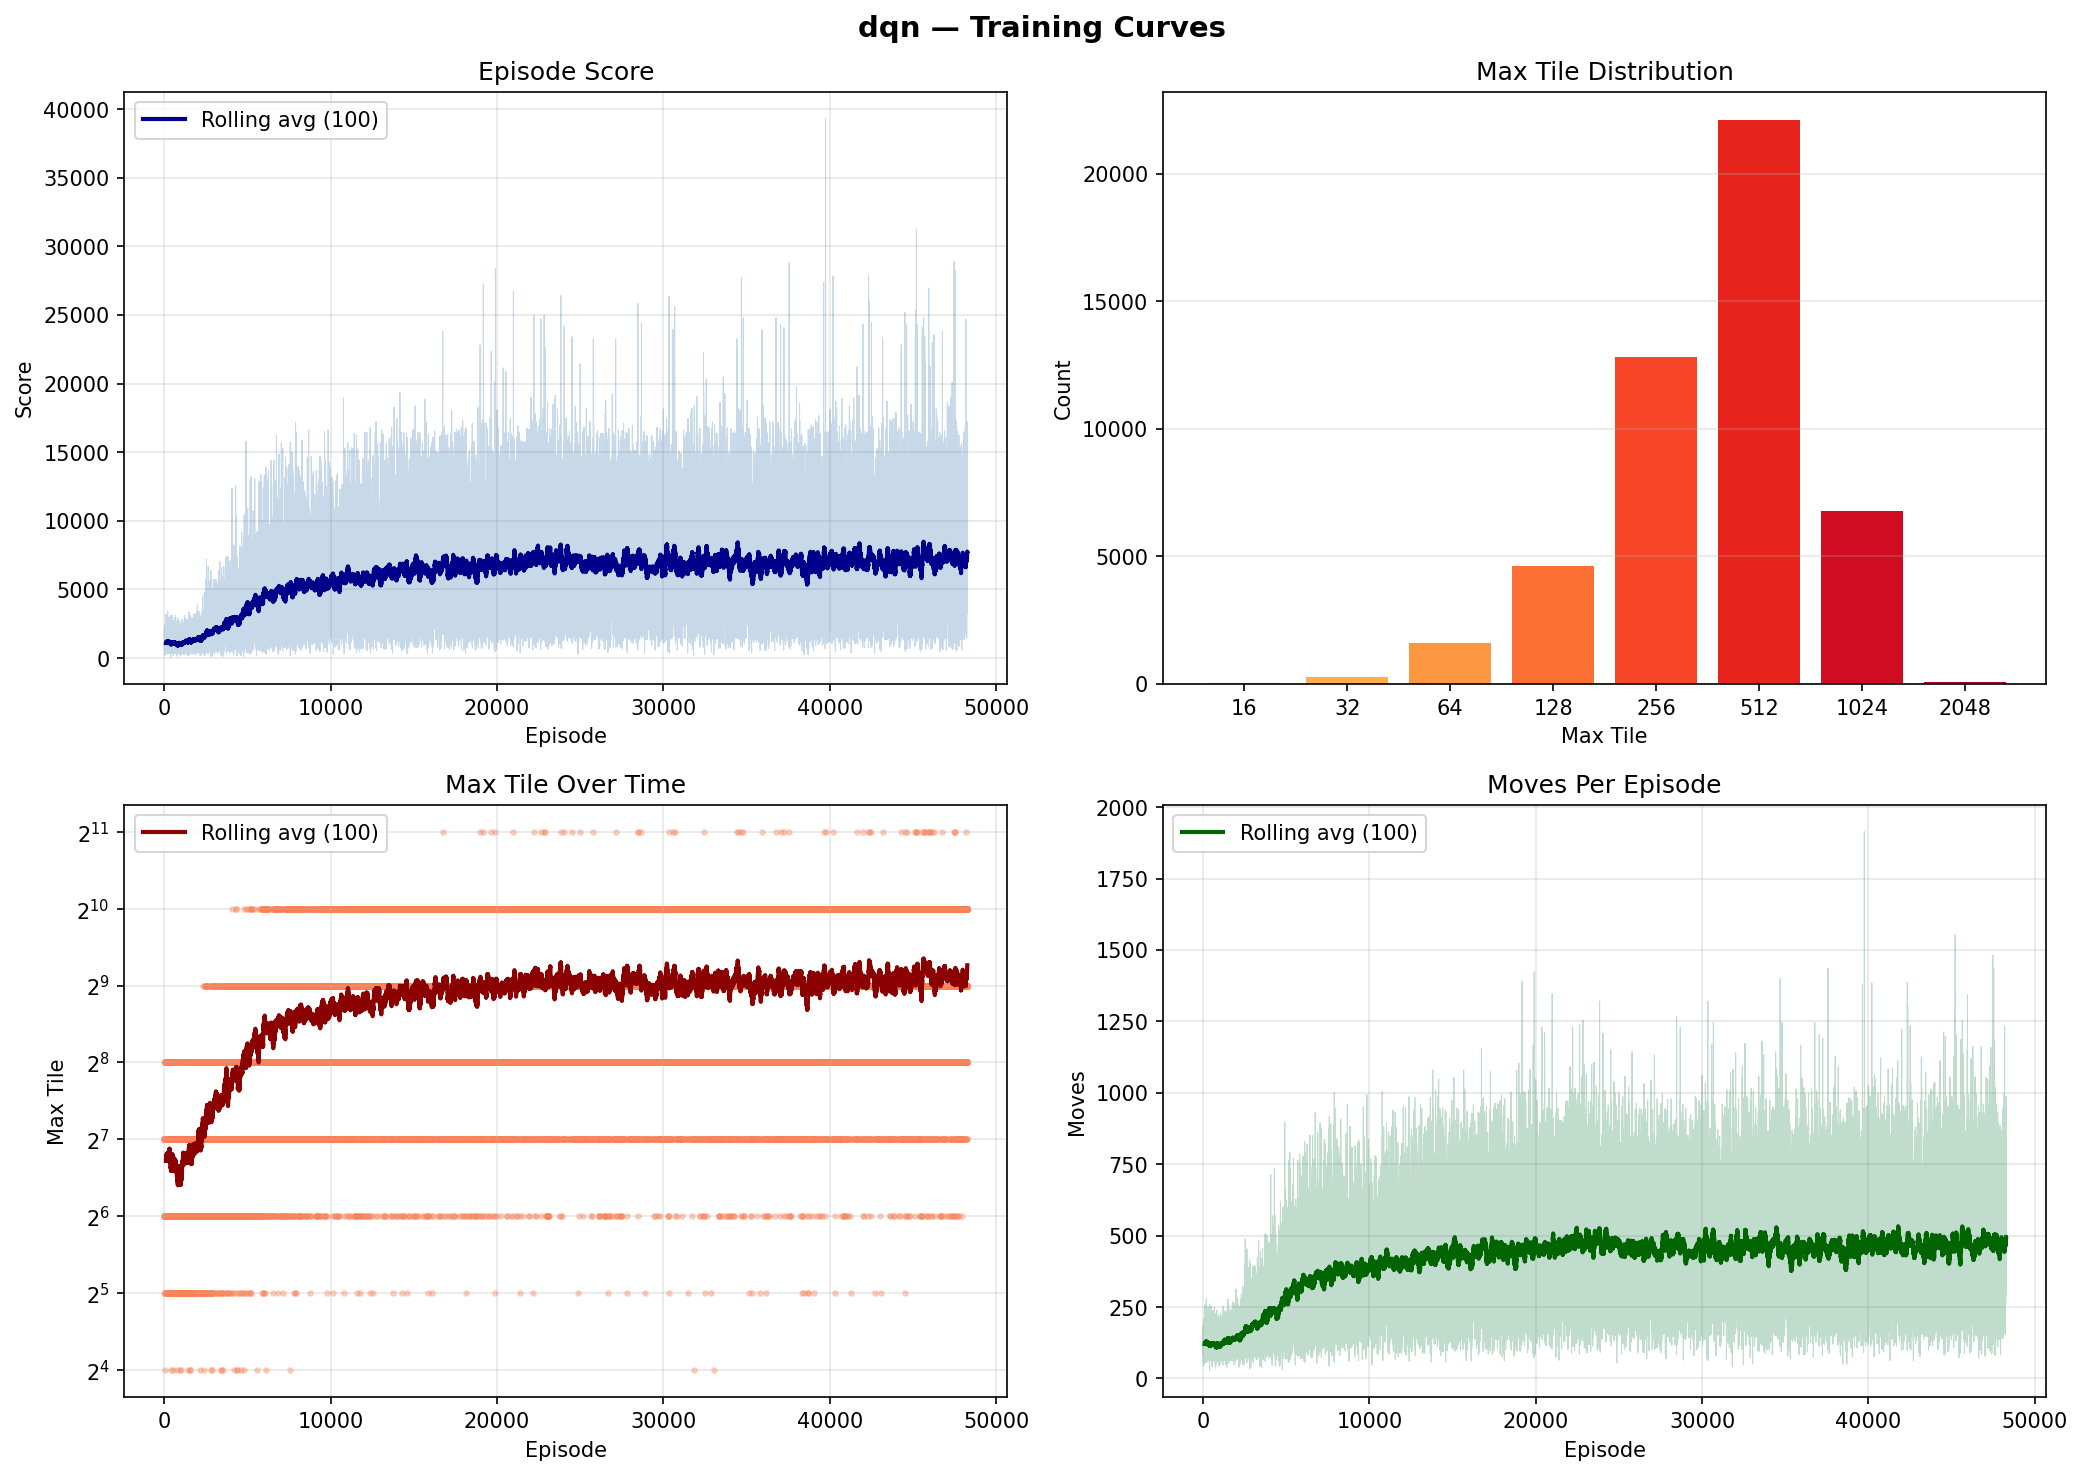
\includegraphics[width=\linewidth]{fig_dqn_5m.png}\\[-3pt]
{\tiny\bfseries\color{accent} DQN $|$ 7,744}
\end{minipage}
\hfill
\begin{minipage}[t]{0.16\linewidth}
\centering
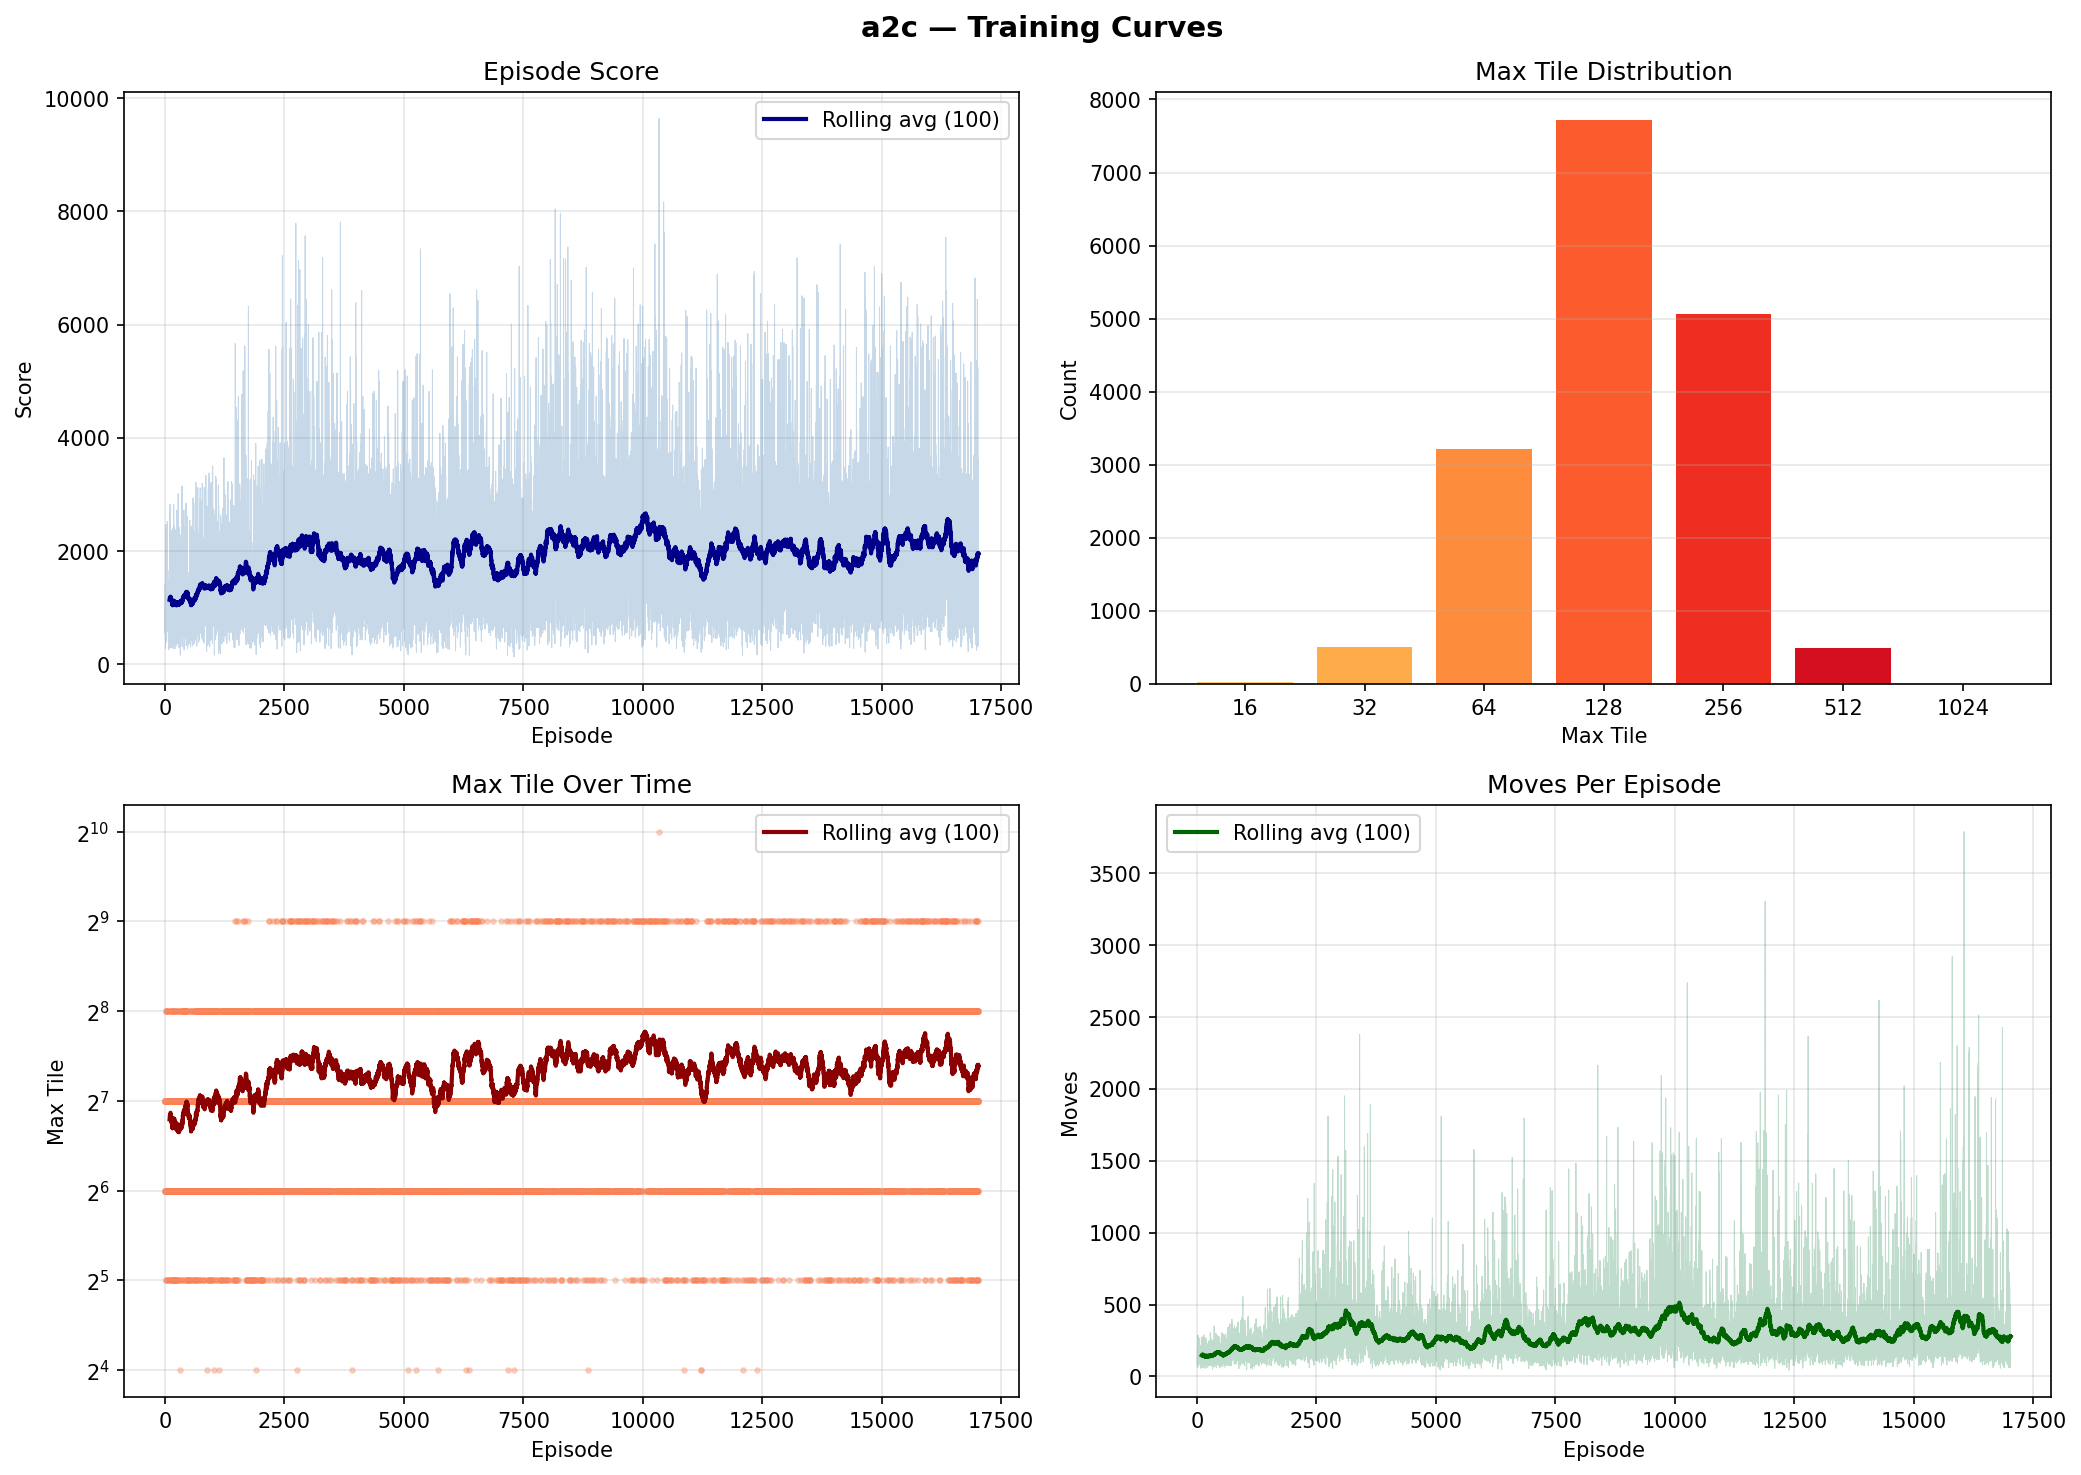
\includegraphics[width=\linewidth]{fig_a2c_5m.png}\\[-3pt]
{\tiny\bfseries\color{info} A2C $|$ 1,944}
\end{minipage}
\hfill
\begin{minipage}[t]{0.16\linewidth}
\centering
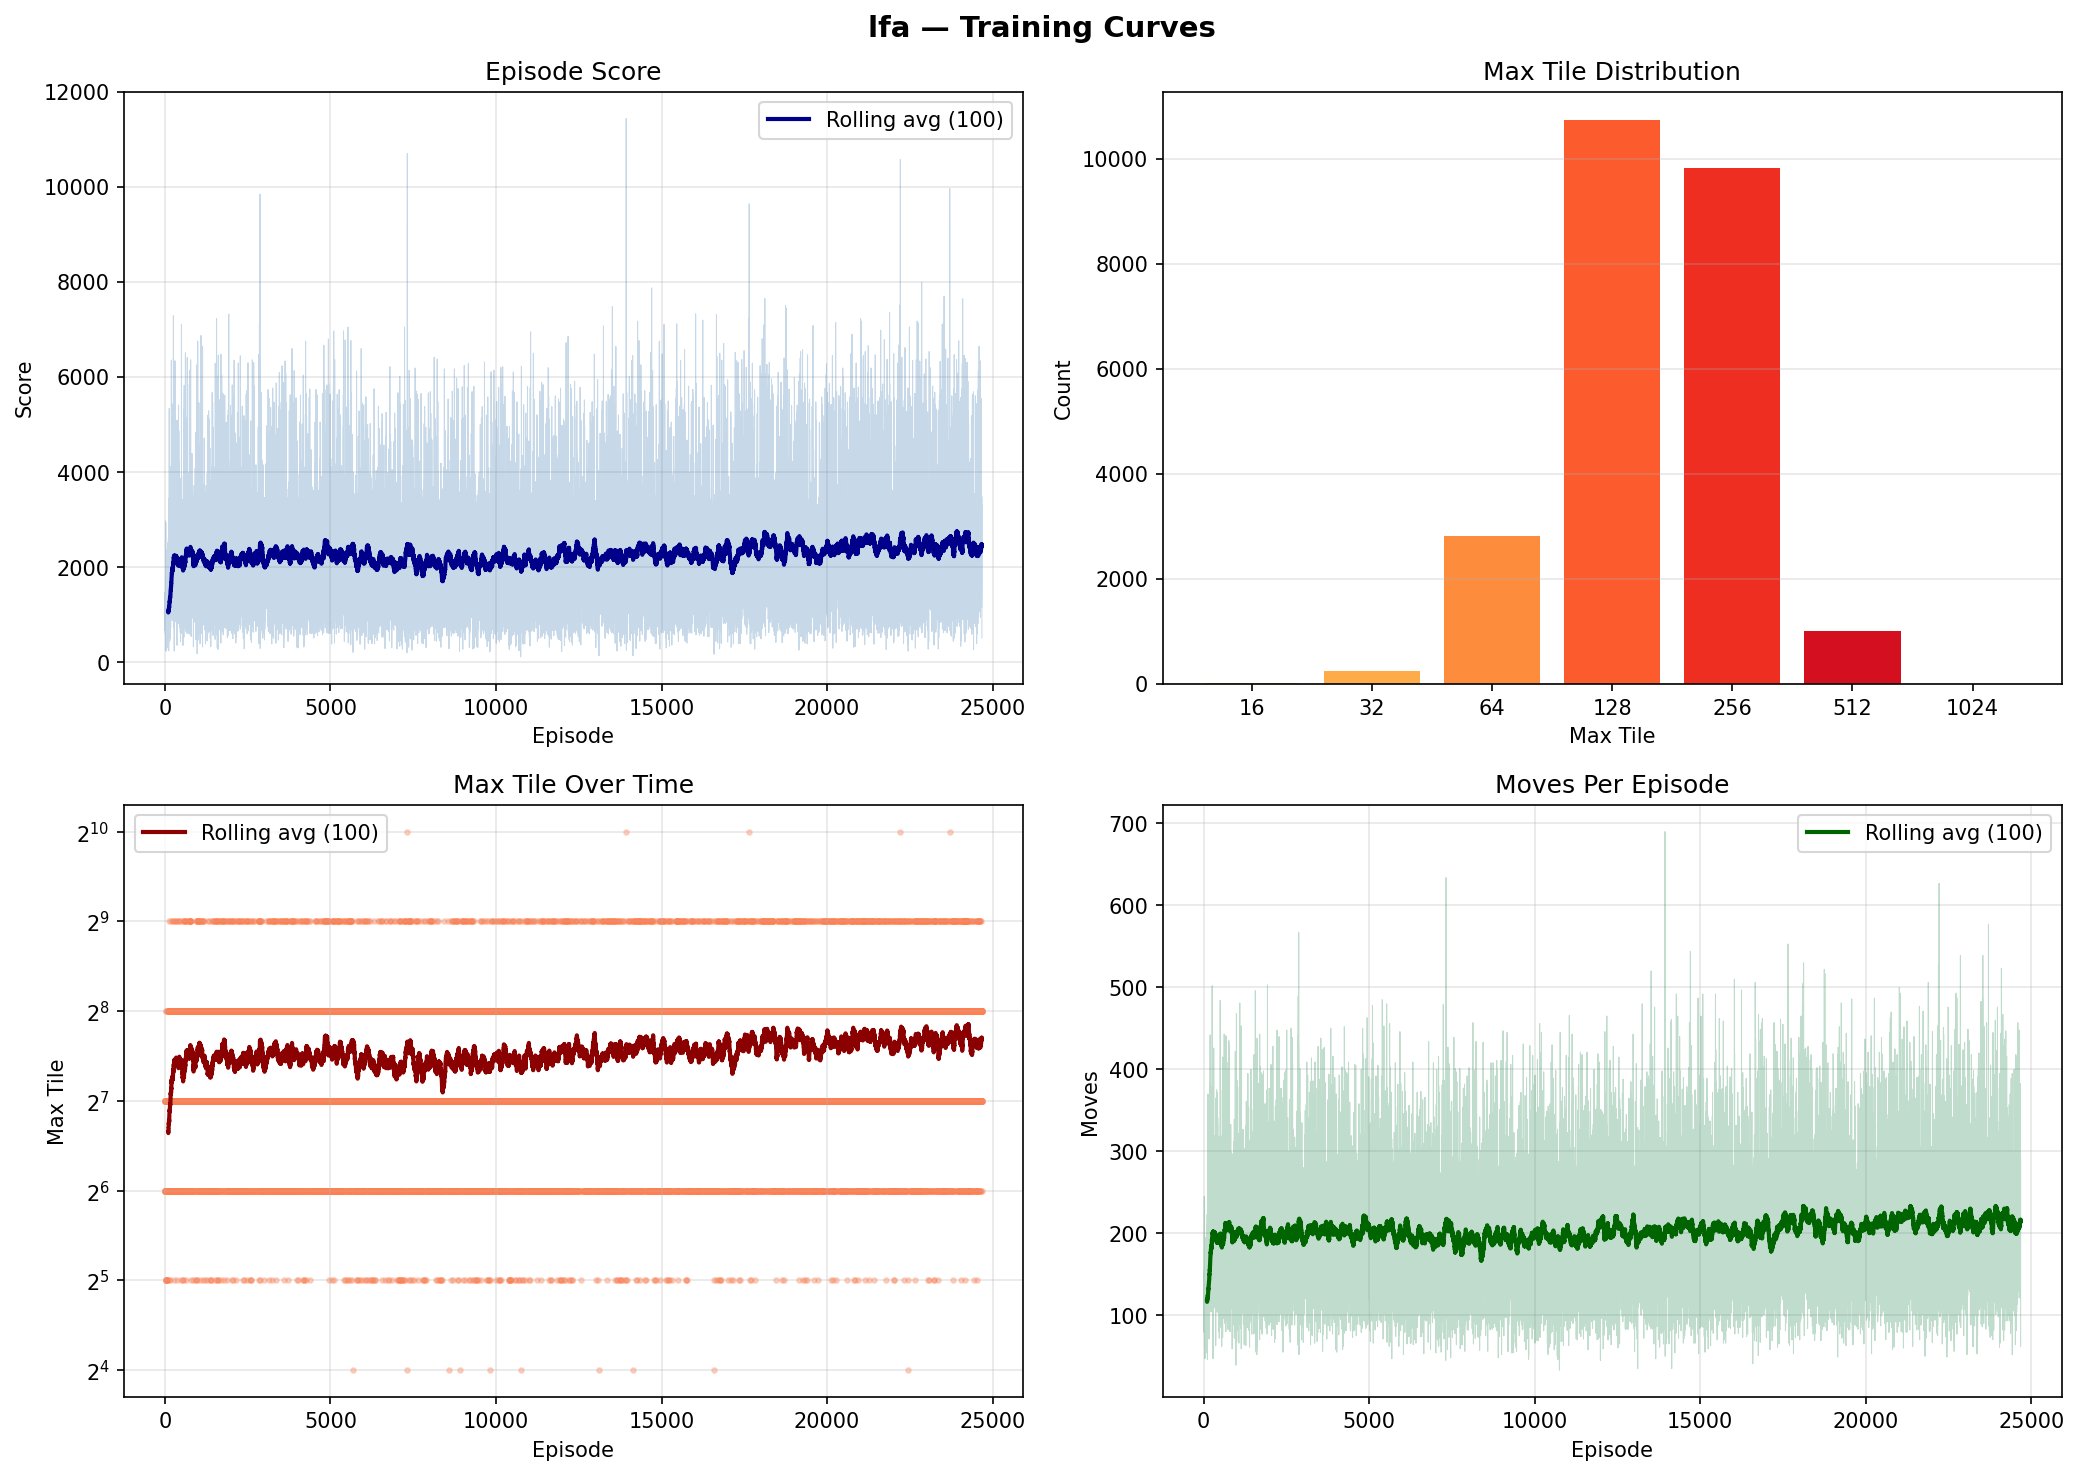
\includegraphics[width=\linewidth]{fig_lfa_5m.png}\\[-3pt]
{\tiny\bfseries\color{success} LFA $|$ 2,456}
\end{minipage}
\hfill
\begin{minipage}[t]{0.16\linewidth}
\centering
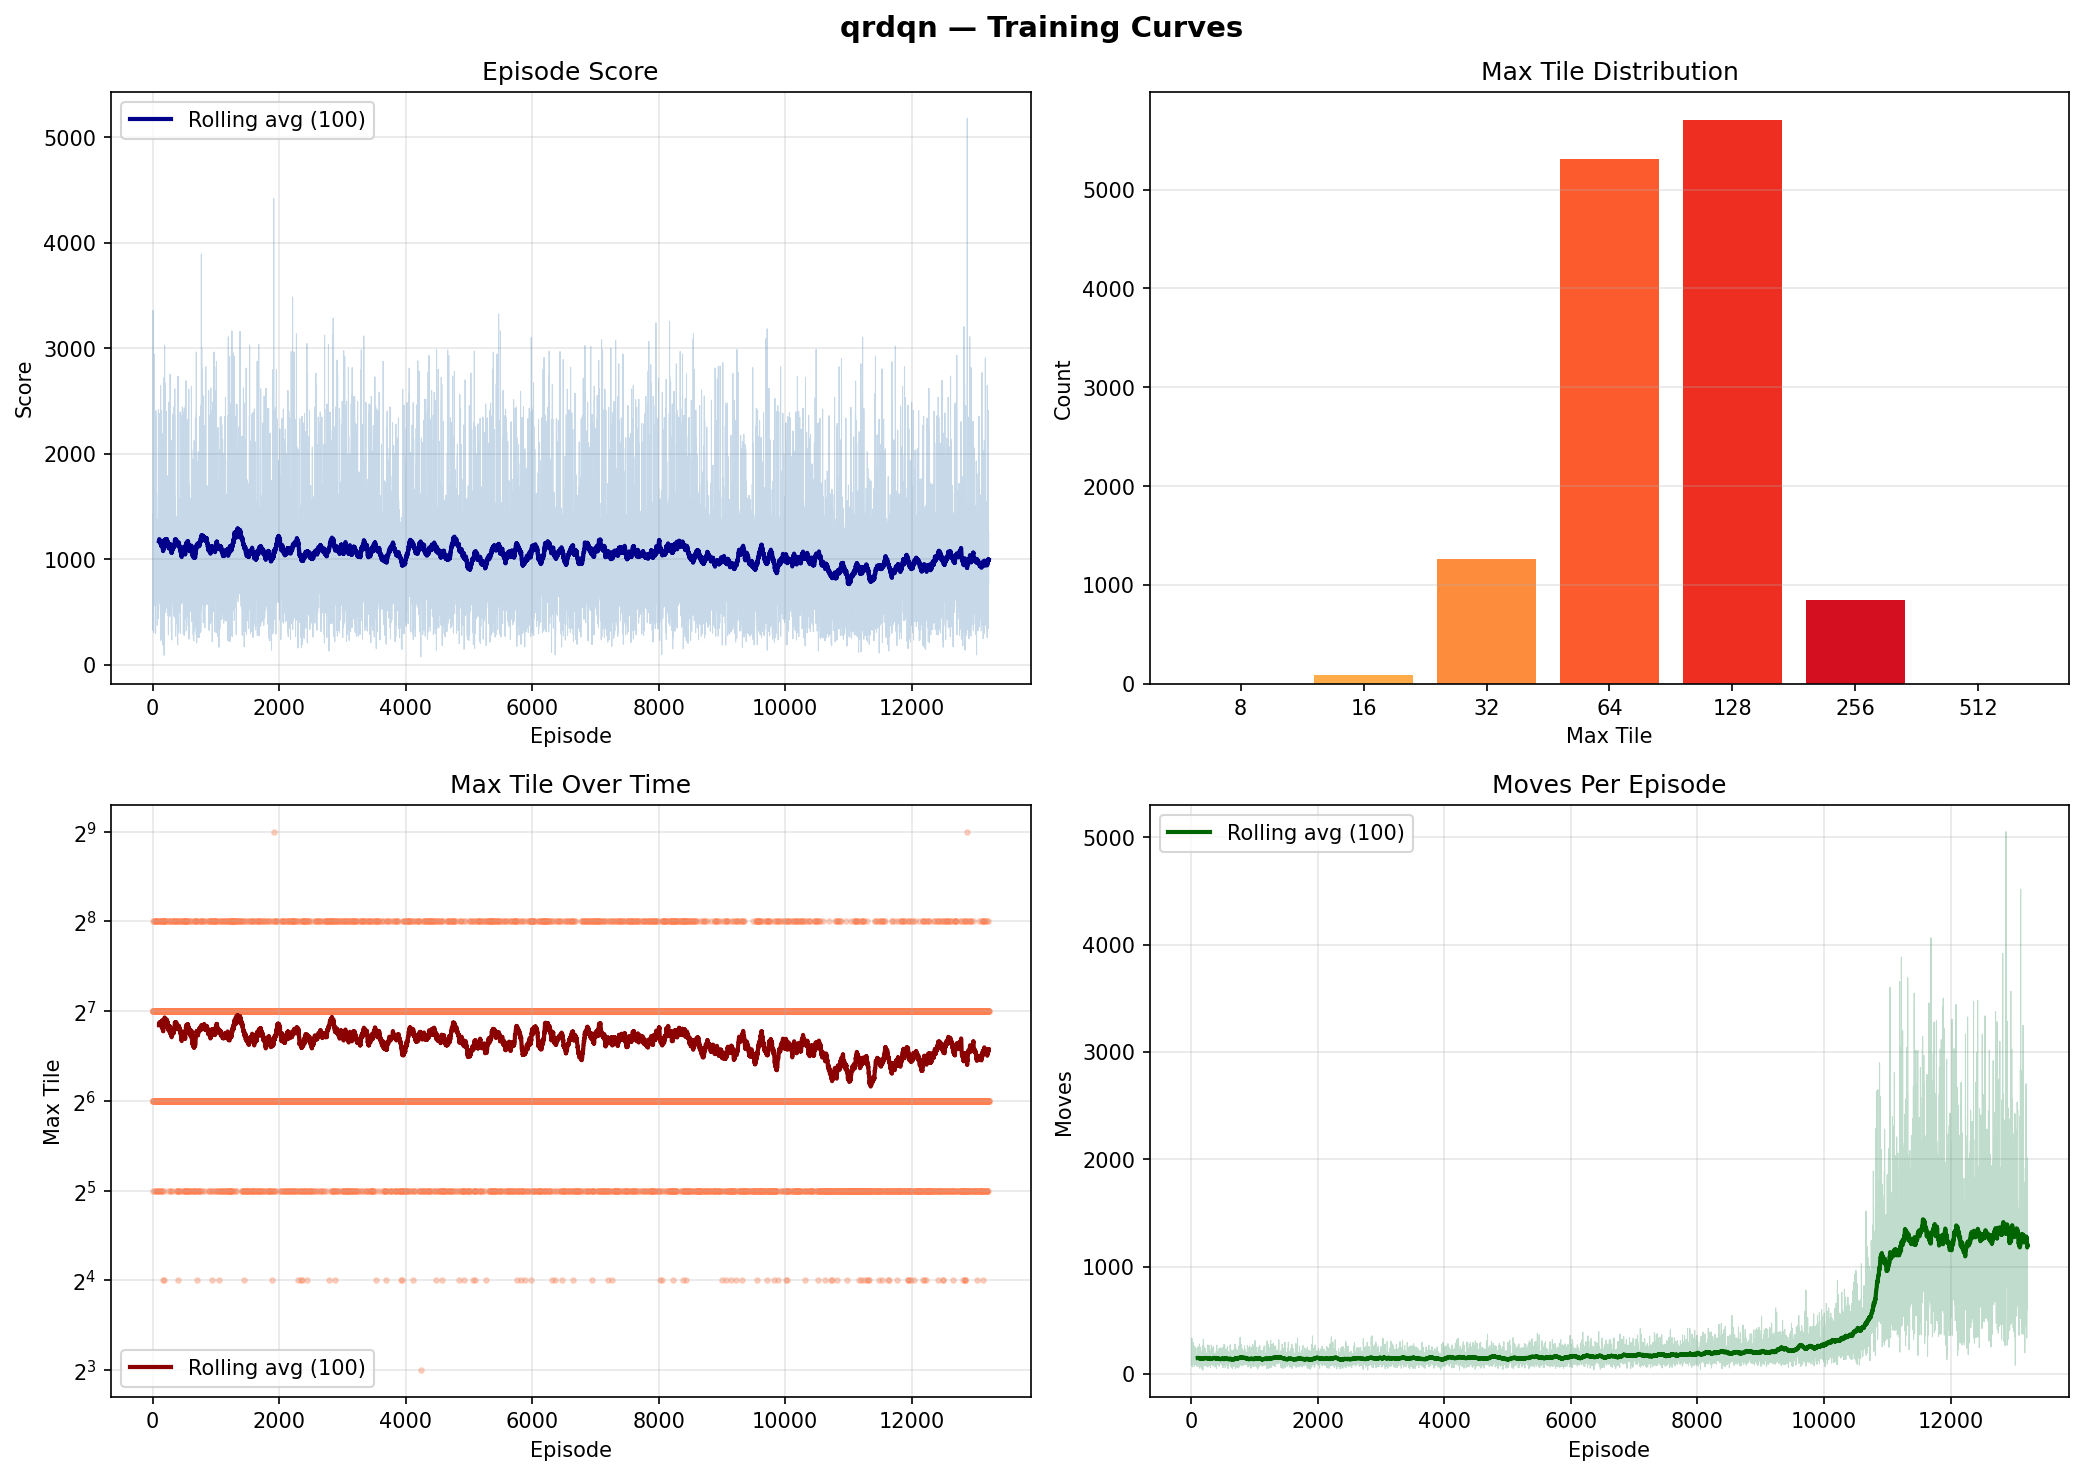
\includegraphics[width=\linewidth]{fig_qrdqn_5m.png}\\[-3pt]
{\tiny\bfseries\color{purple} QR $|$ 995}
\end{minipage}
\hfill
\begin{minipage}[t]{0.16\linewidth}
\centering
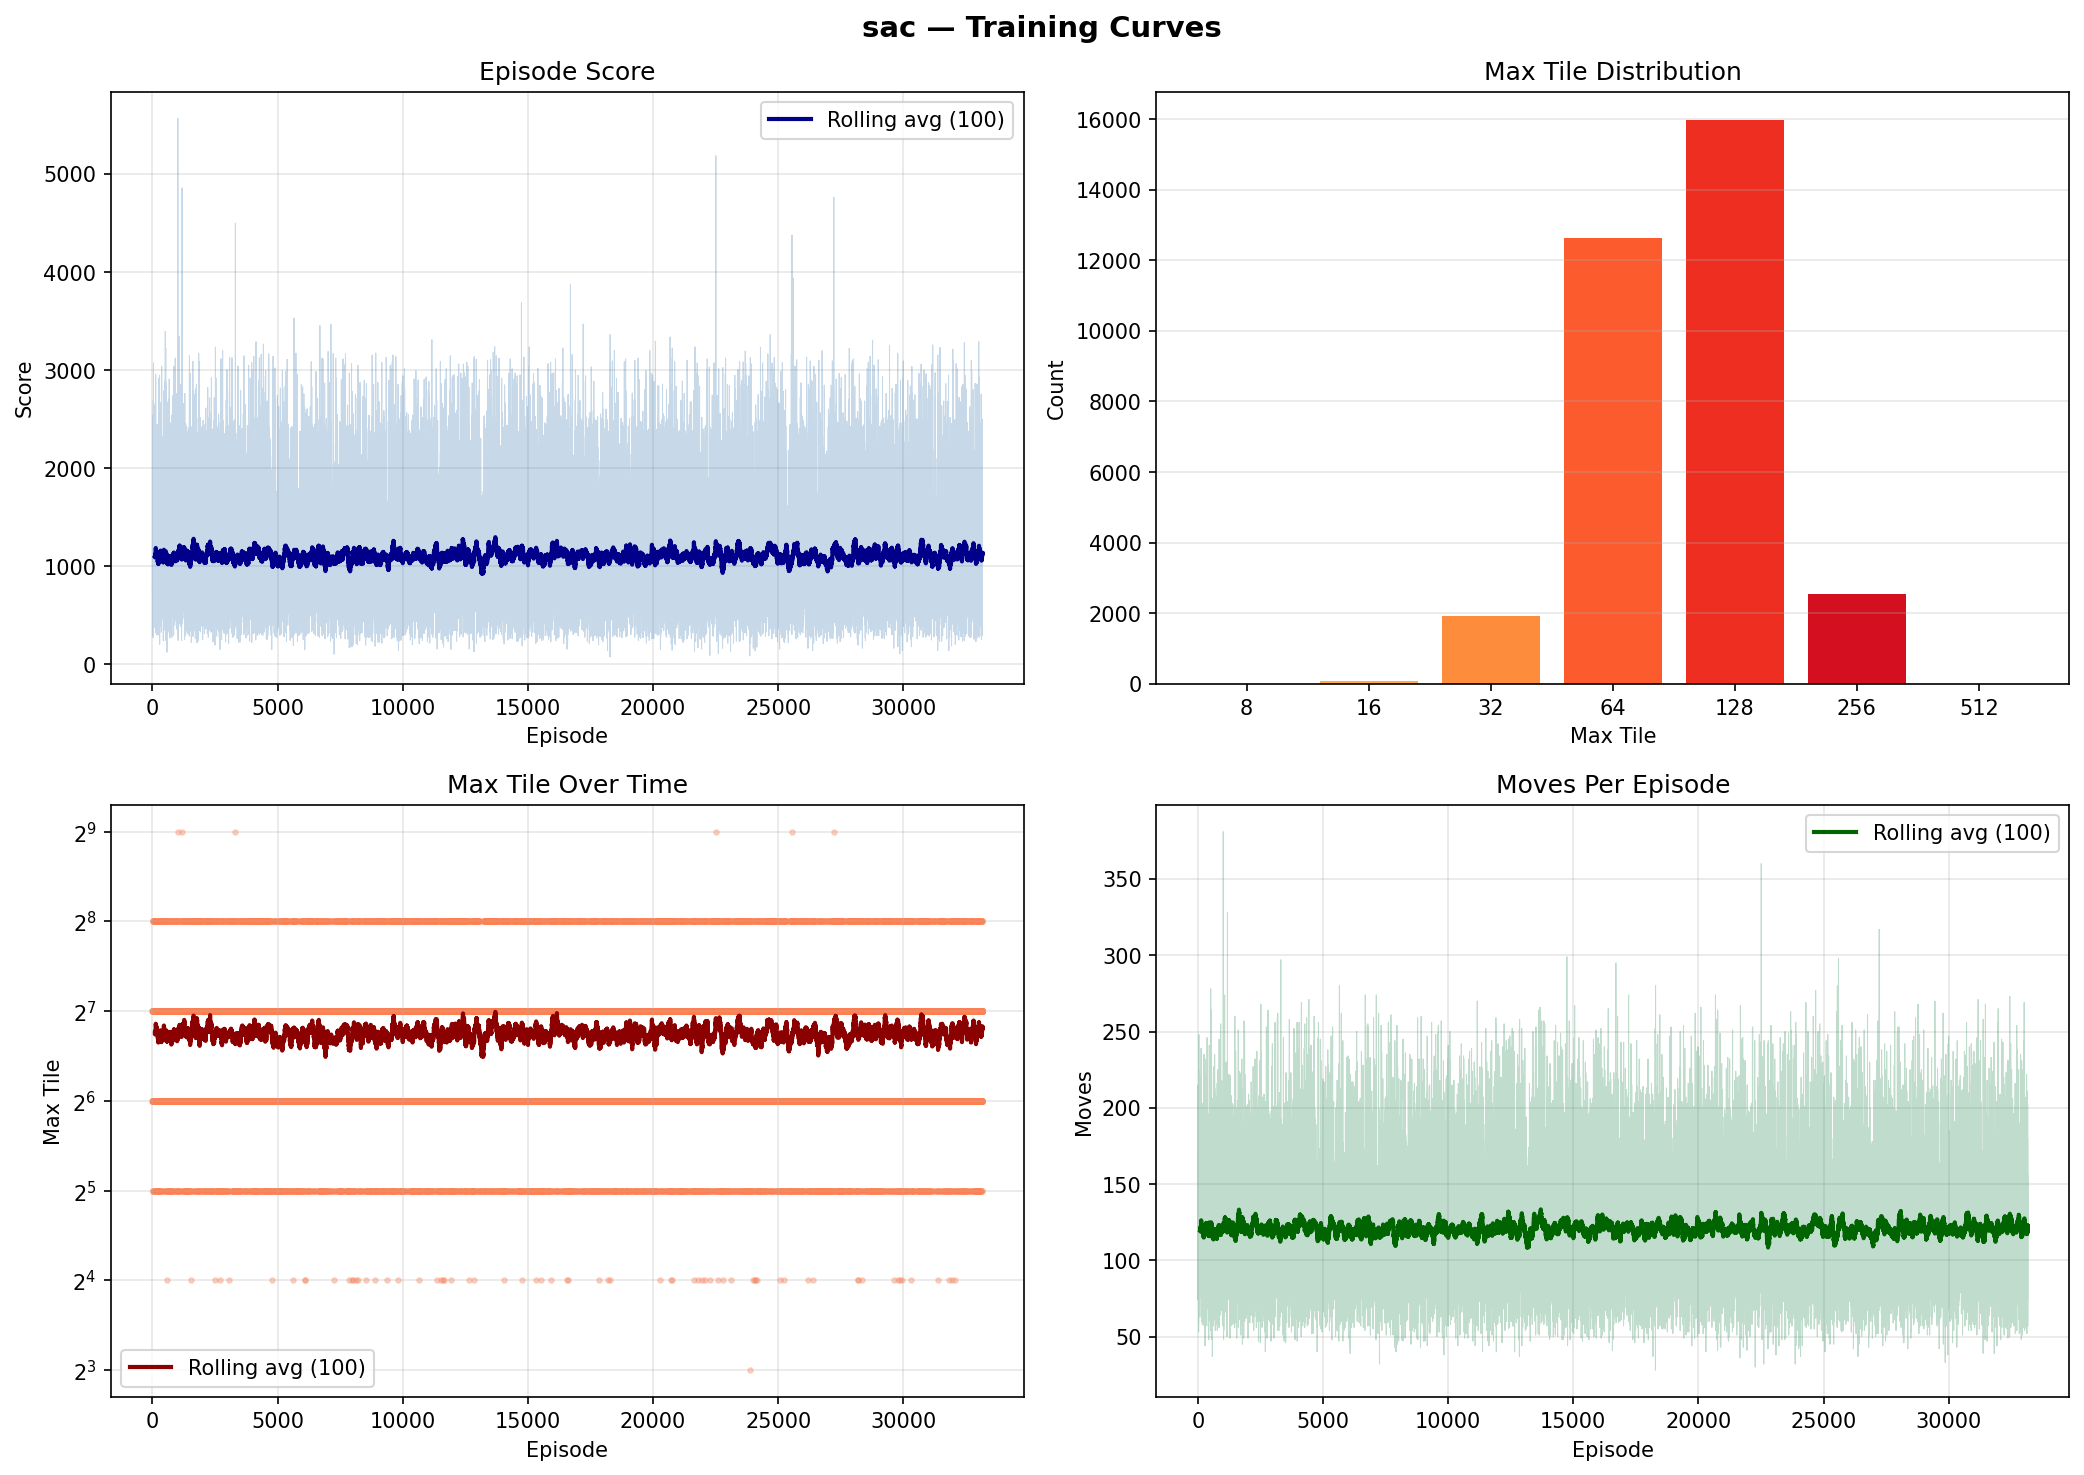
\includegraphics[width=\linewidth]{fig_sac_4m.png}\\[-3pt]
{\tiny\bfseries\color{danger} SAC $|$ 1,131}
\end{minipage}
\hfill
\begin{minipage}[t]{0.16\linewidth}
\centering
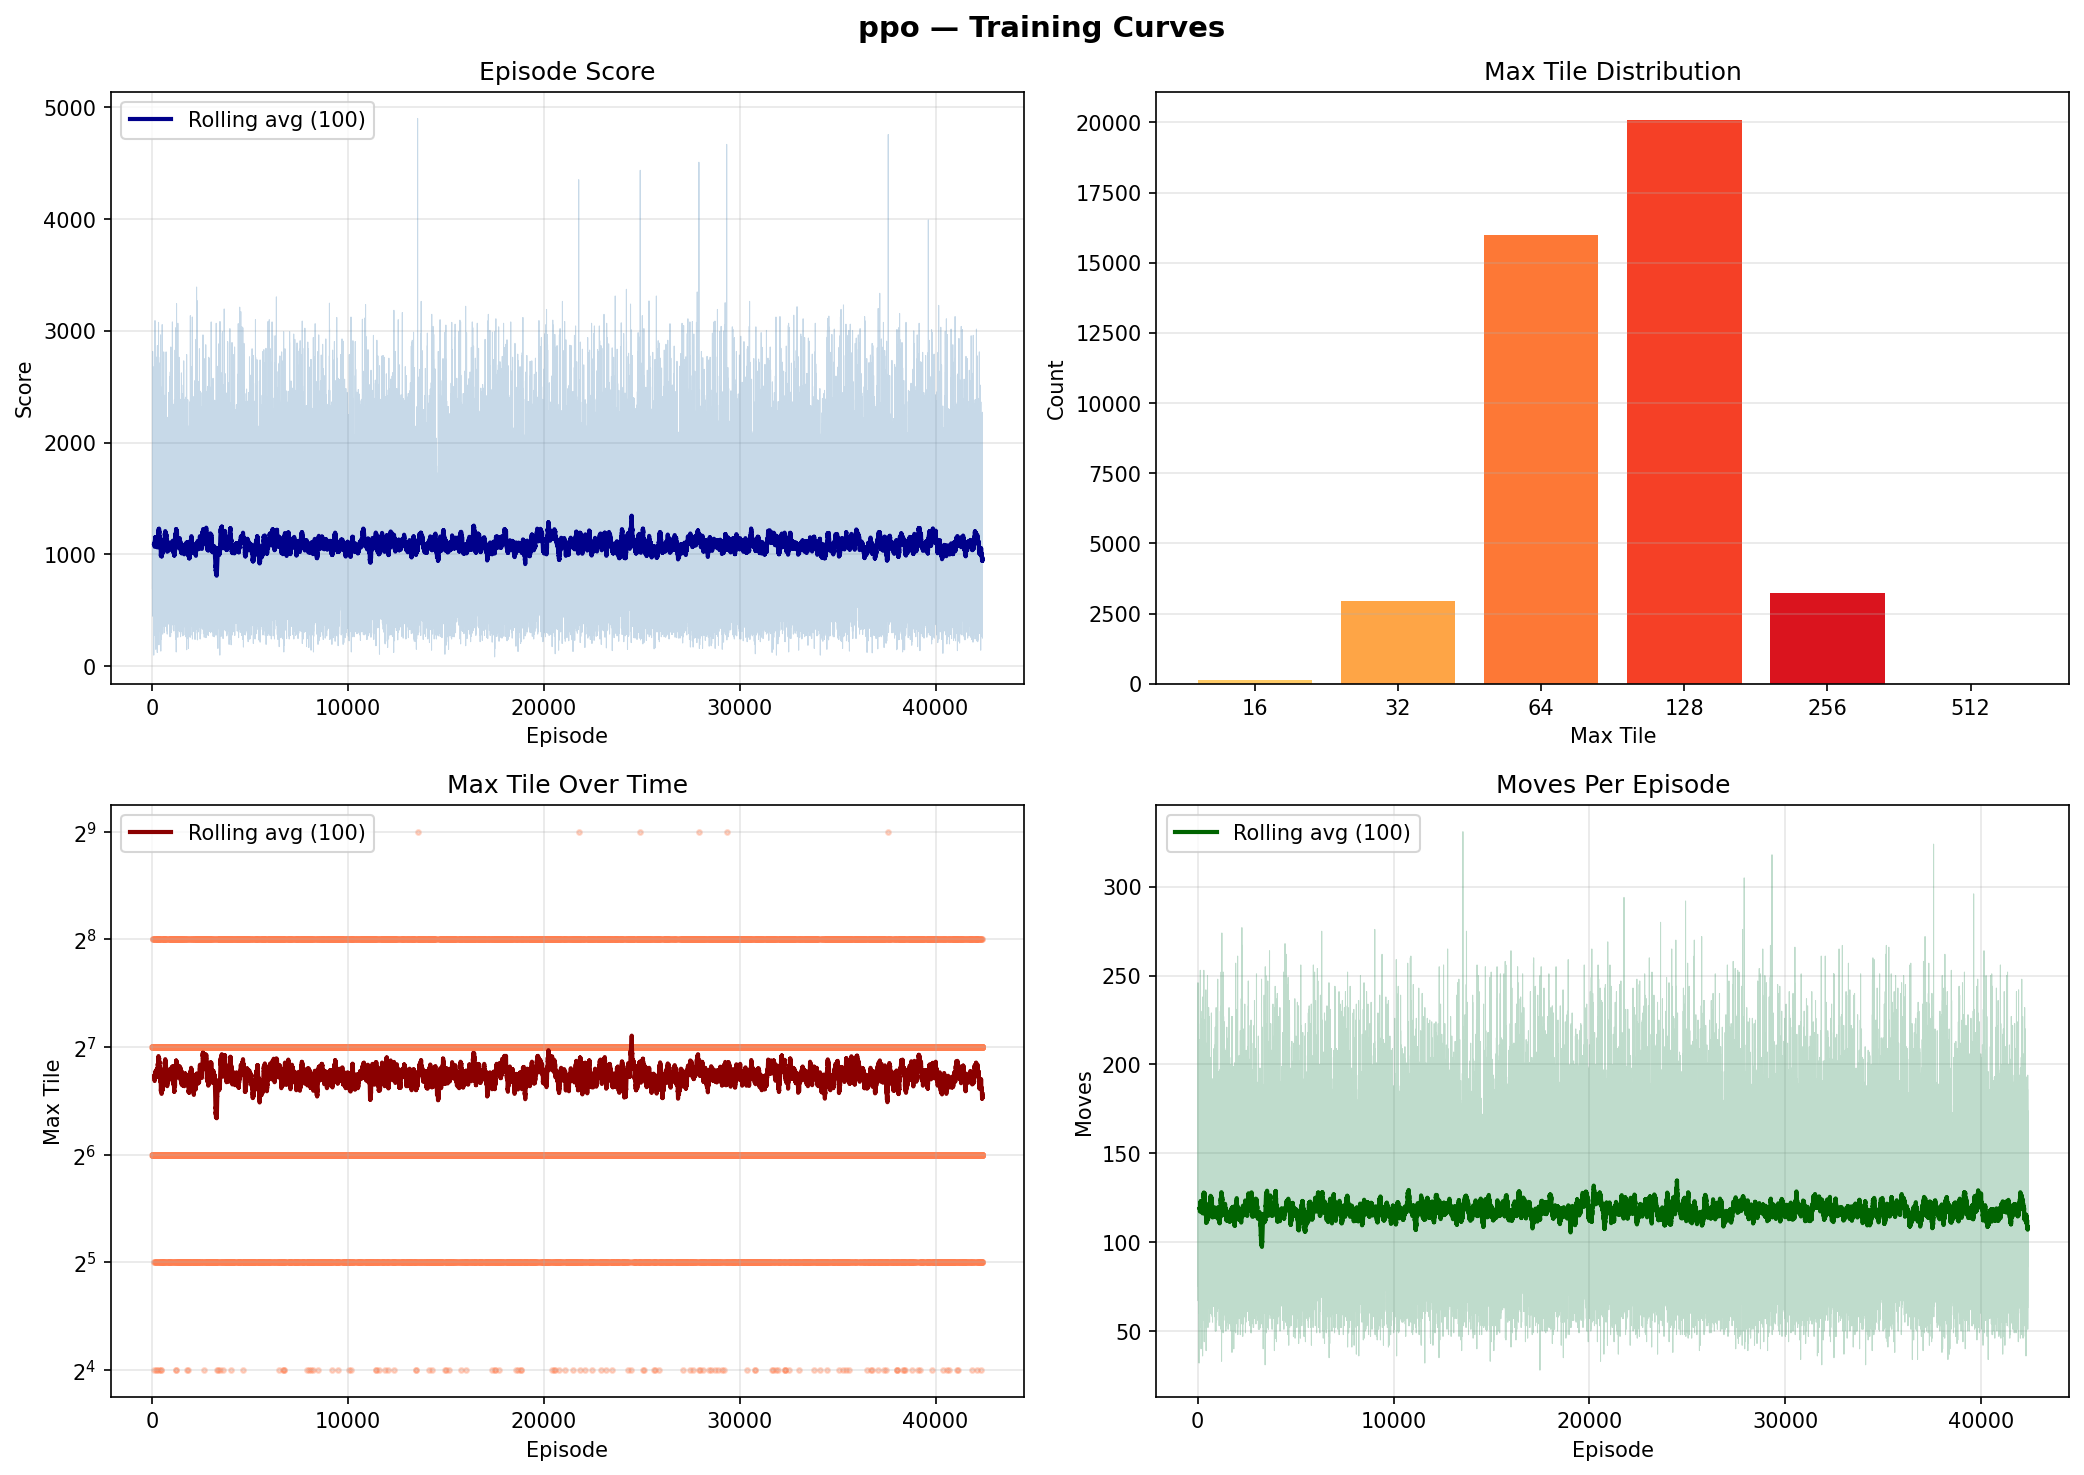
\includegraphics[width=\linewidth]{fig_ppo_5m.png}\\[-3pt]
{\tiny\bfseries\color{info} PPO $|$ 962}
\end{minipage}
\end{center}
\end{sectionbox}

% ─── Bottom Key Insight ────────────────────────────────────────────
\begin{keybox}
\begin{center}
\textbf{Off-policy replay is the decisive factor.} DQN's 100K buffer lets it revisit rare high-scoring trajectories: the key to conquering 2048's sparse rewards.
\end{center}
\end{keybox}

% ═══════════════════════════════════════════════════════════════════
% PAGE 4: ANALYSIS & CONCLUSIONS
% ═══════════════════════════════════════════════════════════════════
\newpage
\pageheader

\pagetitle{Analysis \& Conclusions}{Key insights from 7 agents $\times$ 5M training steps}

\begin{multicols}{2}

% ─── Key Finding 1 ─────────────────────────────────────────────────
\begin{sectionbox}[{\Large\color{white} 1}\; Off-Policy $\gg$ On-Policy]{accent}

\begin{center}
\resizebox{0.85\linewidth}{!}{
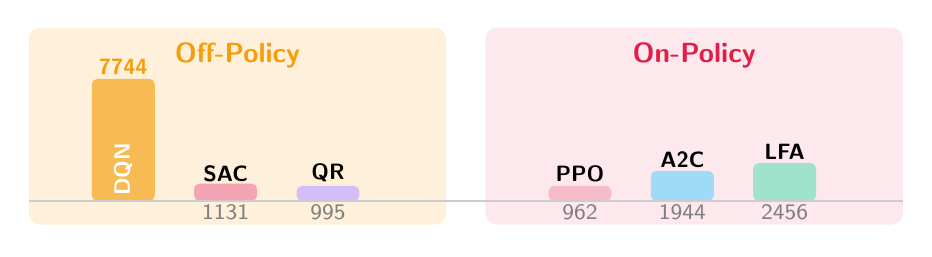
\begin{tikzpicture}
% Off-policy vs on-policy comparison
\fill[accent!15, rounded corners=4pt] (-0.3,-0.3) rectangle (5.0,2.2);
\fill[danger!10, rounded corners=4pt] (5.5,-0.3) rectangle (10.8,2.2);

\node[font=\normalsize\bfseries, text=accent] at (2.35, 1.85) {Off-Policy};
\node[font=\normalsize\bfseries, text=danger] at (8.15, 1.85) {On-Policy};

% DQN bar
\fill[accent!70, rounded corners=2pt] (0.5, 0) rectangle (1.3, 1.55);
\node[font=\footnotesize\bfseries, text=white] at (0.9, 0.4) {\rotatebox{90}{DQN}};
\node[font=\footnotesize\bfseries, text=accent] at (0.9, 1.7) {7744};

% SAC bar
\fill[danger!40, rounded corners=2pt] (1.8, 0) rectangle (2.6, 0.22);
\node[font=\footnotesize\bfseries] at (2.2, 0.35) {SAC};
\node[font=\footnotesize, text=gray] at (2.2, -0.15) {1131};

% QR-DQN bar  
\fill[purple!40, rounded corners=2pt] (3.1, 0) rectangle (3.9, 0.19);
\node[font=\footnotesize\bfseries] at (3.5, 0.35) {QR};
\node[font=\footnotesize, text=gray] at (3.5, -0.15) {995};

% PPO bar
\fill[danger!30, rounded corners=2pt] (6.3, 0) rectangle (7.1, 0.19);
\node[font=\footnotesize\bfseries] at (6.7, 0.35) {PPO};
\node[font=\footnotesize, text=gray] at (6.7, -0.15) {962};

% A2C bar
\fill[info!40, rounded corners=2pt] (7.6, 0) rectangle (8.4, 0.38);
\node[font=\footnotesize\bfseries] at (8.0, 0.52) {A2C};
\node[font=\footnotesize, text=gray] at (8.0, -0.15) {1944};

% LFA bar
\fill[success!40, rounded corners=2pt] (8.9, 0) rectangle (9.7, 0.48);
\node[font=\footnotesize\bfseries] at (9.3, 0.62) {LFA};
\node[font=\footnotesize, text=gray] at (9.3, -0.15) {2456};

\draw[thick, gray!40] (-0.3, 0) -- (10.8, 0);
\end{tikzpicture}
}
\end{center}

{\small
DQN's \textbf{experience replay} (100K buffer) revisits rare high-scoring trajectories thousands of times. On-policy methods discard each trajectory after one update, which is catastrophic for sparse rewards.
}
\end{sectionbox}

% ─── Key Finding 2 ─────────────────────────────────────────────────
\begin{sectionbox}[{\Large\color{white} 2}\; Feature Engineering vs.\ Deep Learning]{success}

\begin{center}
\resizebox{0.85\linewidth}{!}{
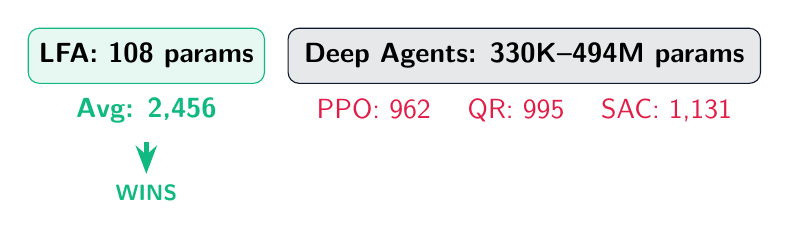
\begin{tikzpicture}
% Parameter efficiency visual
\node[draw=success, fill=success!10, rounded corners=4pt, 
      minimum width=3cm, minimum height=0.7cm, font=\normalsize\bfseries] 
      (lfa) at (0,0) {LFA: 108 params};
\node[draw=primary, fill=primary!10, rounded corners=4pt,
      minimum width=6cm, minimum height=0.7cm, font=\normalsize\bfseries]
      (deep) at (4.8,0) {Deep Agents: 330K--494M params};

\node[font=\normalsize\bfseries, text=success] at (0, -0.7) {Avg: 2,456};
\node[font=\normalsize, text=danger] at (4.8, -0.7) {PPO: 962 \quad QR: 995 \quad SAC: 1,131};

\draw[ultra thick, success, -{Stealth}] (0, -1.1) -- (0, -1.5)
    node[below, font=\footnotesize\bfseries, text=success] {WINS};
\end{tikzpicture}
}
\end{center}

{\small
Hand-crafted monotonicity \& corner features provide stronger inductive bias than CNNs learning from scratch. \textbf{4000$\times$ parameter efficiency!} But LFA plateaus at ${\sim}2500$ (linear capacity ceiling).
}
\end{sectionbox}

% ─── Key Finding 3 ─────────────────────────────────────────────────
\begin{sectionbox}[{\Large\color{white} 3}\; Scaling Reveals Divergent Trajectories]{info}

\renewcommand{\arraystretch}{1.2}
{\small
\begin{tabular}{@{}ccl@{}}
\toprule
\textbf{Pattern} & \textbf{$\Delta$} & \textbf{Agents} \\
\midrule
\textcolor{accent}{\textbf{$\uparrow$ Strong}} & \textcolor{accent}{\textbf{+174\%}} & DQN \\
\textcolor{info}{$\uparrow$ Modest} & +56--62\% & A2C, SAC \\
\textcolor{gray}{$\rightarrow$ Plateau} & +7\% & LFA \\
\textcolor{danger}{\textbf{$\downarrow$ Degrade}} & \textcolor{danger}{\textbf{$-$9--12\%}} & PPO, QR-DQN \\
\bottomrule
\end{tabular}
}

\vspace{4pt}
{\small More training doesn't always help! PPO \emph{gets worse} with 5$\times$ more data. QR-DQN develops invalid-move loops (moves/episode: 200 $\to$ 1000+).}
\end{sectionbox}

\columnbreak

% ─── Key Finding 4 ─────────────────────────────────────────────────
\begin{sectionbox}[{\Large\color{white} 4}\; Exploration Breaks Policy Cycles]{danger}

\begin{center}
\resizebox{0.85\linewidth}{!}{
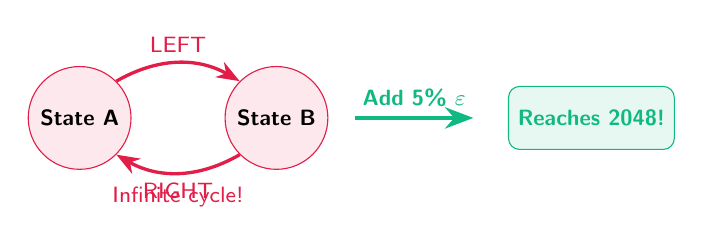
\begin{tikzpicture}
% Cycle diagram
\node[draw=danger, fill=danger!10, circle, minimum size=1cm, font=\footnotesize\bfseries] (s1) at (0,0) {State A};
\node[draw=danger, fill=danger!10, circle, minimum size=1cm, font=\footnotesize\bfseries] (s2) at (2.5,0) {State B};

\draw[-{Stealth}, very thick, danger] (s1.north east) to[bend left=30] node[above, font=\footnotesize] {LEFT} (s2.north west);
\draw[-{Stealth}, very thick, danger] (s2.south west) to[bend left=30] node[below, font=\footnotesize] {RIGHT} (s1.south east);

\node[font=\footnotesize, text=danger] at (1.25, -1.0) {Infinite cycle!};

% Solution
\draw[-{Stealth}, ultra thick, success] (3.5, 0) -- (5.0, 0) node[midway, above, font=\footnotesize\bfseries] {Add 5\% $\varepsilon$};

\node[draw=success, fill=success!10, rounded corners=4pt, 
      minimum width=2cm, minimum height=0.8cm, font=\footnotesize\bfseries, text=success] at (6.5, 0) {Reaches 2048!};
\end{tikzpicture}
}
\end{center}

{\small
Deterministic greedy policies repeat suboptimal moves at high-tile states. Just \textbf{5\% random noise} breaks cycles $\to$ DQN reaches 2048 in Hunt mode.
}
\end{sectionbox}

% ─── Key Finding 5 ─────────────────────────────────────────────────
\begin{sectionbox}[{\Large\color{white} 5}\; GRPO: Model Scale $\to$ Board Reasoning]{purple}

\begin{center}
\resizebox{0.85\linewidth}{!}{
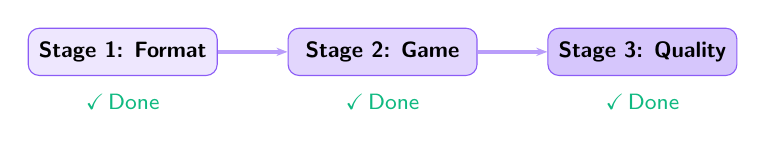
\begin{tikzpicture}[
    stage/.style={rectangle, rounded corners=4pt, draw=purple, fill=#1,
                  minimum width=2.4cm, minimum height=0.6cm, font=\footnotesize\bfseries},
    arr/.style={-{Stealth[length=4pt]}, very thick, purple!60}
]
\node[stage=purple!15] (s1) at (0,0) {Stage 1: Format};
\node[stage=purple!25] (s2) at (3.3,0) {Stage 2: Game};
\node[stage=purple!35] (s3) at (6.6,0) {Stage 3: Quality};

\draw[arr] (s1) -- (s2);
\draw[arr] (s2) -- (s3);

\node[font=\footnotesize, text=success, below=3pt of s1] {\checkmark\,Done};
\node[font=\footnotesize, text=success, below=3pt of s2] {\checkmark\,Done};
\node[font=\footnotesize, text=success, below=3pt of s3] {\checkmark\,Done};
\end{tikzpicture}
}
\end{center}

{\small
\textbf{Scaling results:} 0.5B $\to$ score 704, tile 64 \quad|\quad \textbf{1.5B $\to$ score 2,348, tile 256}

3$\times$ more parameters $\to$ 3.3$\times$ higher score. Larger models reason about board merges; 0.5B memorizes format but can't plan.
}
\end{sectionbox}

% ─── Latency ───────────────────────────────────────────────────────
\begin{sectionbox}[{\raisebox{-1pt}{\tikz\fill[info] (0,0) rectangle (0.35,0.35);}\; Inference Latency}]{info}
\begin{center}
\resizebox{0.85\linewidth}{!}{
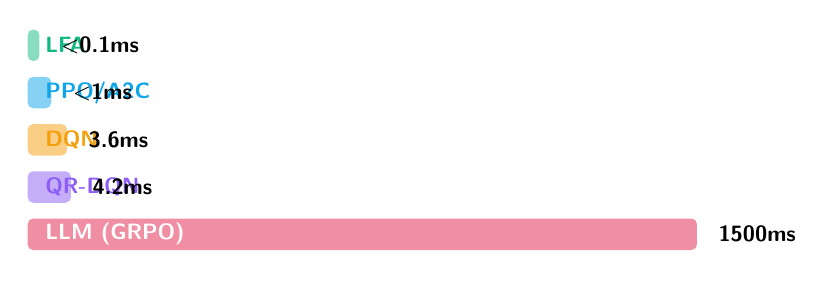
\begin{tikzpicture}
% Latency bars - manual
\fill[success!50, rounded corners=2pt] (0,0) rectangle (0.15,0.4);
\node[font=\footnotesize\bfseries, anchor=west, text=success] at (0.1,0.2) {LFA};
\node[font=\footnotesize\bfseries, anchor=west] at (0.3,0.2) {$<$0.1ms};
%
\fill[info!50, rounded corners=2pt] (0,-0.6) rectangle (0.3,-0.2);
\node[font=\footnotesize\bfseries, anchor=west, text=info] at (0.1,-0.4) {PPO/A2C};
\node[font=\footnotesize\bfseries, anchor=west] at (0.45,-0.4) {$<$1ms};
%
\fill[accent!50, rounded corners=2pt] (0,-1.2) rectangle (0.5,-0.8);
\node[font=\footnotesize\bfseries, anchor=west, text=accent] at (0.1,-1.0) {DQN};
\node[font=\footnotesize\bfseries, anchor=west] at (0.65,-1.0) {3.6ms};
%
\fill[purple!50, rounded corners=2pt] (0,-1.8) rectangle (0.55,-1.4);
\node[font=\footnotesize\bfseries, anchor=west, text=purple] at (0.1,-1.6) {QR-DQN};
\node[font=\footnotesize\bfseries, anchor=west] at (0.7,-1.6) {4.2ms};
%
\fill[danger!50, rounded corners=2pt] (0,-2.4) rectangle (8.5,-2.0);
\node[font=\footnotesize\bfseries, anchor=west, text=white] at (0.1,-2.2) {LLM (GRPO)};
\node[font=\footnotesize\bfseries, anchor=west] at (8.65,-2.2) {1500ms};
\end{tikzpicture}
}
\end{center}

{\small LLM is \textbf{400$\times$ slower} but provides \textbf{interpretable} chain-of-thought reasoning.}
\end{sectionbox}

% ─── Future Work ───────────────────────────────────────────────────
\begin{sectionbox}[{\raisebox{-1pt}{\tikz\fill[primary] (0,0) rectangle (0.35,0.35);}\; Future Work}]{primary}
\begin{itemize}[nosep, leftmargin=10pt, itemsep=2pt]
    \item[\textcolor{accent}{$\triangleright$}] Scale GRPO to Qwen2.5-3B / 7B (A100 GPU)
    \item[\textcolor{accent}{$\triangleright$}] Scaling curves at checkpoints 50K$\to$5M
    \item[\textcolor{accent}{$\triangleright$}] Multi-seed experiments for error bars
    \item[\textcolor{accent}{$\triangleright$}] Hybrid LLM-MCTS exploration
    \item[\textcolor{accent}{$\triangleright$}] Longer GRPO max\_completion for deeper reasoning
\end{itemize}
\end{sectionbox}

\end{multicols}

% ─── Conclusions Banner ────────────────────────────────────────────
\begin{keybox}
\begin{center}
{\large\bfseries Key Takeaways}\\[4pt]
{\small
\textcolor{accent}{\textbf{1.}} DQN dominates (avg 7,744, tile 2048) via experience replay \quad
\textcolor{success}{\textbf{2.}} LFA (108 params) beats all deep on-policy agents \quad
\textcolor{info}{\textbf{3.}} PPO degrades with more training\\
\textcolor{purple}{\textbf{4.}} GRPO 1.5B reaches tile 256 (3.3$\times$ better than 0.5B) \quad
\textcolor{danger}{\textbf{5.}} 5\% exploration noise is essential for reaching 2048
}
\end{center}
\end{keybox}

\vspace{2pt}
\begin{center}
{\footnotesize\color{gray} CS 5180 $|$ Prof.\ Robert Platt $|$ Khoury College, Northeastern University \quad|\quad Hardware: NVIDIA RTX 4060 (8\,GB), CUDA 12.6}
\end{center}

\end{document}
